%    Copyright (C) 2012  L. Schmid
%
%    This file is free: you can redistribute it and/or modify
%    it under the terms of the GNU General Public License as published by
%    the Free Software Foundation, either version 3 of the License, or
%    (at your option) any later version, but you have to reference to the original owner.
%
%	 Additionaly the authors have to be readable in the final document.
%
%    This program is distributed in the hope that it will be useful,
%    but WITHOUT ANY WARRANTY; without even the implied warranty of
%    MERCHANTABILITY or FITNESS FOR A PARTICULAR PURPOSE.  See the
%    GNU General Public License for more details.
%
%    You should have received a copy of the GNU General Public License
%    along with this program.  If not, see <http://www.gnu.org/licenses/>.

%%%%%%%%%%%%%%%%%%%%%%%% 
% Dokumentinformationen %
%%%%%%%%%%%%%%%%%%%%%%%%%
\newcommand{\titleinfo}{TSM\_AdvContr}
\newcommand{\authorinfo}{L. Schmid / H. Diethelm / J. Perdrizat}  % Do not remove any names! Initial authors stay first.
\newcommand{\versioninfo}{$Revision: 1424 $ - powered by \LaTeX}

%%%%%%%%%%%%%%%%%%%%%%%%%%%%%%%%%%%%%%%%%%%%%
% Standard projektübergreifender Header für
% - Makros 
% - Farben
% - Mathematische Operatoren
%
% DORT NUR ERGÄNZEN, NICHTS LÖSCHEN
%%%%%%%%%%%%%%%%%%%%%%%%%%%%%%%%%%%%%%%%%%%%%
% Genereller Header
\documentclass[10pt,twoside,a4paper,fleqn]{article}
\usepackage[utf8]{inputenc}
\usepackage[left=1cm,right=1cm,top=1cm,bottom=1cm,includeheadfoot]{geometry}
\usepackage[ngerman]{babel,varioref}

% Pakete
\usepackage{amssymb,amsmath,fancybox,graphicx,color,lastpage,wrapfig,fancyhdr,hyperref,verbatim,floatflt,multirow,rotating,tabularx,enumitem,subfig,siunitx,pdfpages}


%%%%%%%%%%%%%%%%%%%%
% Generelle Makros %
%%%%%%%%%%%%%%%%%%%%
\newcommand{\formelbuch}[1]{\footnotesize{(Skript S. #1)}\normalsize{}}
\newcommand{\verweis}[2]{\small{(siehe auch \ref{#1}, #2 (S. \pageref{#1}))}}
\newcommand{\subsubadd}[1]{\textcolor{black}{\mbox{#1}}}

\newcommand{\matlab}[1]{\footnotesize{(Matlab: \texttt{#1})}\normalsize{}}


\newenvironment{liste}[0]{
	\begin{list}{$\bullet$}{ \leftmargin=0.5cm \setlength{\itemsep}{0cm}\setlength{\parsep}{0cm} \setlength{\topsep}{0cm}}}
  {\end{list}}
\newenvironment{aufzaehlung}[0]{
    \begin{enumerate}\setlength{\leftmargin=0.5cm \itemsep}{1pt}\setlength{\parskip}{0pt}\setlength{\parsep}{0pt}}
  {\end{enumerate}}      

\newcommand{\abbHeight}[3]{
	\begin{center}
		\includegraphics[height=#2]{./bilder/#1} \\
		#3
    \end{center}
}

%%%%%%%%%%
% Farben %
%%%%%%%%%%
\definecolor{black}{rgb}{0,0,0}
\definecolor{red}{rgb}{1,0,0}
\definecolor{white}{rgb}{1,1,1}
\definecolor{grey}{rgb}{0.8,0.8,0.8}

%%%%%%%%%%%%%%%%%%%%%%%%%%%%
% Mathematische Operatoren %
%%%%%%%%%%%%%%%%%%%%%%%%%%%%
\DeclareMathOperator{\sinc}{sinc}



% Fouriertransformationen
\unitlength1cm
\newcommand{\FT}
{
\begin{picture}(1,0.5)
\put(0.2,0.1){\circle{0.14}}\put(0.27,0.1){\line(1,0){0.5}}\put(0.77,0.1){\circle*{0.14}}
\end{picture}
}
\newcommand{\DFT}
{
\overset{DFT}{
	\begin{picture}(1,0.2)
	\put(0.2,0.1){\circle{0.14}}{\put(0.27,0.1){\line(1,0){0.5}}}\put(0.77,0.1){\circle*{0.14}}
	\end{picture}
}
}


\newcommand{\IFT}
{
\begin{picture}(1,0.5)
\put(0.2,0.1){\circle*{0.14}}\put(0.27,0.1){\line(1,0){0.45}}\put(0.77,0.1){\circle{0.14}}
\end{picture}
}

\newcommand{\IDFT}
{
\overset{IDFT}{
    \begin{picture}(1,0.2)
	\put(0.2,0.1){\circle*{0.14}}\put(0.27,0.1){\line(1,0){0.45}}\put(0.77,0.1){\circle{0.14}}
	\end{picture}
}
}



%%%%%%%%%%%%%%%%%%%%%%%%%%%%
% Allgemeine Einstellungen %
%%%%%%%%%%%%%%%%%%%%%%%%%%%%
%pdf info
\hypersetup{pdfauthor={\authorinfo},pdftitle={\titleinfo},colorlinks=false}
\author{\authorinfo}
\title{\titleinfo}

%Kopf- und Fusszeile
\pagestyle{fancy}
\fancyhf{}
%Linien oben und unten
\renewcommand{\headrulewidth}{0.5pt} 
\renewcommand{\footrulewidth}{0.5pt}

\fancyhead[L]{\titleinfo{ }\tiny{(\versioninfo)}}
%Kopfzeile rechts bzw. aussen
\fancyhead[R]{Seite \thepage { }von \pageref{LastPage}}
%Fusszeile links bzw. innen
\fancyfoot[L]{\footnotesize{\authorinfo}}
%Fusszeile rechts bzw. ausen
\fancyfoot[R]{\footnotesize{\today}}

% Einrücken verhindern versuchen
\setlength{\parindent}{0pt}


%%============Aufzählungen===========%%
%%=======\usepackage{enumitem}=======%%
\setlist{itemsep=-2pt}
\setlist{parsep=-2pt}


% Möglichst keine Ergänzungen hier, sondern in header.tex
\begin{document}
\tableofcontents
\newpage
\section{Zustandsraumdarstellung \tiny{$Revision: 1352 $}}
\scriptsize
\label{sec:ZRD}

\subsection{Basics}
Darstellung einer Differentialgleichung $n$. Ordnung durch ein
Differentialgleichungssystem von $n$ Gleichungen 1. Ordnung.


\begin{figure}[!h]
	\normalsize
	\begin{minipage}{.45\linewidth}
		\centering
		\normalsize
		\subfloat{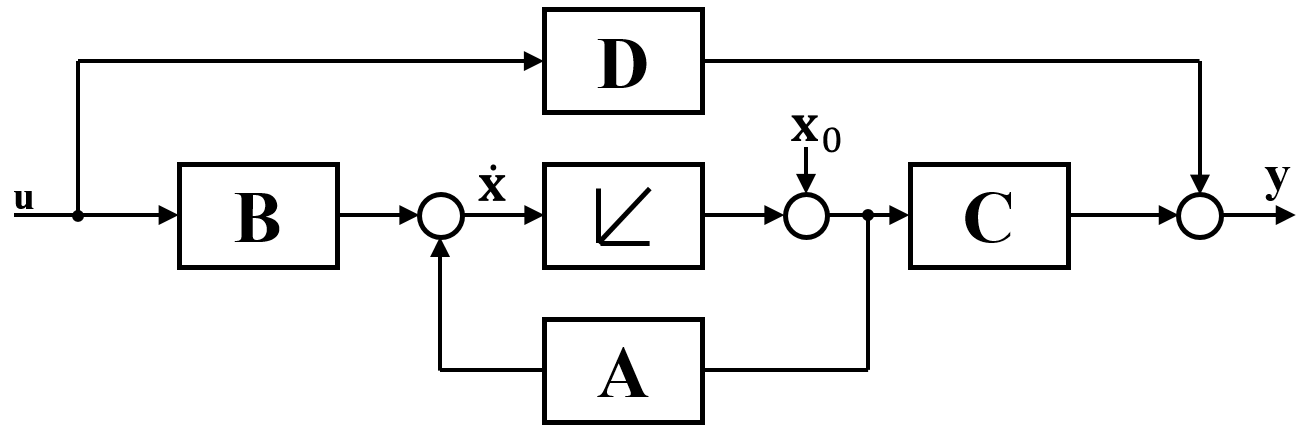
\includegraphics[width=\linewidth]{./bilder/zrd.png}}
	\end{minipage}%
	\hfill
	\begin{minipage}{.45\linewidth}
		$\dot{\underline{x}}(t) = {\boldsymbol A} \underline{x}(t) + {\boldsymbol B}
		\underline{u}(t)$\newline
		$\underline{y}(t) = {\boldsymbol C} \underline{x}(t) + {\boldsymbol D}
		\underline{u}(t)$\\ \\
		Pole des Systems: Eigenwerte von $\boldsymbol{A}$\\
		$\det\left(\lambda \boldsymbol{I}- \boldsymbol{A}\right) =0$
	\end{minipage}
	\caption{Zustandsraumdarstellung}
	\label{fig:ZRD}
\end{figure}



\begin{tabularx}{\linewidth}{lllX}\hline
	\textbf{Matrix}			&\textbf{Dimension}		&\textbf{Einfluss}					&\textbf{Weiteres}\\\hline
	${\boldsymbol A}$		&$n \times n$			&Beschreibt Dynamik des Systems 	& Spalten entsprechen Ausgängen der Intergratoren\newline Zeilen deren Eingänge\\\hline
	${\boldsymbol B}$		&$n \times M$			&Einfluss der Eingangsvariablen auf Zustandsvariablen 	& Steuer- oder Eingangsmatrix\\\hline
	${\boldsymbol C}$		&$P \times n$			&Einfluss der Zustandsvariablen auf Ausgangsgrössen		& Beobachtungs- oder Ausgangsmatrix\\\hline
	${\boldsymbol D}$		&$P \times M$			&Direkter Einfluss der Eingangsvariablen auf Ausgangsvariablen & Übergangs- oder Durchgangsmatrix\\\hline
\end{tabularx}\\
Dabei gilt:\hspace{5mm}
$n$ = Anzahl Zustandsvariablen; \hspace{5 mm}
$M$ = Anzahl Eingangsvariablen; \hspace{5 mm}
$P$ = Anzahl Ausgangsvariablen
\subsubsection{Stabilität}
Ein LTI-System ist asymptotisch stabil wenn der Realanteil aller Eigenwerte von A kleiner als Null ist. Die Impulsantwort klingt dann gegen Null ab.
\subsubsection{MIMO-Systeme}
\begin{itemize}
	\item Bei einem MIMO-System ist $\boldsymbol{G}\left(s\right)$ eine $P\times M$-Matrix
	\begin{itemize}
		\item Dabei beschreibt jede der Übertragungsfunktionen den Einfluss eines Eingangs auf den  Ausgang
		\item Somit gilt: \begin{equation*}
		\boldsymbol{G}\left( s \right) = \begin{bmatrix}
		\text{Einfluss Eingang 1 auf Ausgang 1}		&	\text{Einfluss Eingang 2 auf Ausgang 1}&	\cdots& \text{Einfluss Eingang M auf Ausgang 1}\\
		\text{Einfluss Eingang 1 auf Ausgang 2}		&	\text{Einfluss Eingang 2 auf Ausgang 2}& \cdots& \text{Einfluss Eingang M auf Ausgang 2}\\
		\vdots										&	\vdots									&\cdots&	\vdots								\\
		\text{Einfluss Eingang 1 auf Ausgang P}		&	\text{Einfluss Eingang 2 auf Ausgang P}& \cdots &\text{Einfluss Eingang M auf Ausgang P}\\
		\end{bmatrix}
		\end{equation*}
	\end{itemize}
\end{itemize}

\subsection{ZRD zu Übertragungsfunktion (im Bildbereich) }

\begin{equation}
\label{eq:ss2tf}
	\boldsymbol{G}\left( s \right) = \frac{\boldsymbol{Y}\left( s \right)}{\boldsymbol{U}\left( s\right)} = \boldsymbol{C}\left( s\boldsymbol{I}-\boldsymbol{A}\right)^{-1}\boldsymbol{B}+\boldsymbol{D} = \frac{b_{m} s^{m} + b_{m-1} s^{m-1} +\cdots+b_{1} s + b_{0}}{s^{n} + a_{n-1} s^{n-1} + \cdots + a_{1} s + a_{0}}
\end{equation}
\begin{itemize}
	\item Dabei ist $\boldsymbol{I}$ die Einheitsmatrix mit der Dimension von $\boldsymbol{A}$
	\item  Wenn $\boldsymbol{D} \neq 0$, dann ist $b_m \neq 0$ und die Sprungantwort des Systems hat eine Sprungkomponente im Ausgang.
	\item Vorteilhaft in TR: Aus multiplizieren mit Variablen, nicht mit eingesetzten Werten um frühzeitiges Kürzen zu verhindern.
\end{itemize}

\subsection{Übertragungsfunktion zu ZRD}
\begin{itemize}
	\item Matlab: \textit{ss2tf}
	\item Es sind verschiedene Umformungen möglich, sie können die Steuerbarkeit ()\ref{subsubsec:Steuerbarkeit}) oder die Beobachtbarkeit (\ref{subsubsec:Beobachtbarkeit}) garantieren. Für beide oft verwendeten Umformungen muss $G\left( s\right)$ in folgende Form gebracht werden:
\end{itemize}
\begin{equation*}
	G \left( s\right) = \frac{b_{n-1}\cdot s^{n-1}+\ldots+b_1\cdot s+b_0}{s^n+a_{n-1}\cdot s^{n-1}+\ldots+a_1\cdot s+a_0}+d
\end{equation*}
\subsubsection{Steuerbare kanonische Normalform}
Mit dieser Methode umgeformte Systeme sind immer steuerbar
\begin{eqnarray} \nonumber
\boldsymbol{A}_c = 
	\begin{bmatrix}
		0 		& 1 		& 0 		&\cdots & 0\\
		0 		& 0 		& 1 		&\cdots & 0\\
		\vdots	& \ddots	& \ddots	&\ddots	& \vdots\\
		0		&\cdots		&0			&\cdots &1\\
		-a_0	&-a_1		&-a_2		&\cdots	&-a_{n-1}
	\end{bmatrix} &
\boldsymbol{B}_c = 
	\begin{bmatrix}
		0\\
		0\\
		\vdots\\
		0\\
		1
	\end{bmatrix} &
\boldsymbol{C}_c = 
	\begin{bmatrix}
		b_0	& b_1 & b_2 &\cdots &b_{n-1}	
	\end{bmatrix} \hspace{5mm}
	D_c = d
\end{eqnarray}

\subsubsection{Beobachtbare kanonische Normalform}
Mit dieser Methode umgeformte Systeme sind immer beobachtbar
\begin{eqnarray} \nonumber
\boldsymbol{A}_c = 
	\begin{bmatrix}
		0 		& 0 		& \cdots  	&0 		& -a_0\\
		1 		& 0 		& \cdots 	&0 		& -a_1\\
		0		&1			&\cdots 	&0 		& -a_2\\
		\vdots	& \ddots	& \ddots	&\vdots	& \vdots\\
		0		&0			&\cdots		&1		&-a_{n-1}
	\end{bmatrix} &
\boldsymbol{B}_o = 
		\begin{bmatrix}
		b_0\\
		b_1\\
		\vdots\\
		b_{n-2}\\
		b_{n-1}
	\end{bmatrix} &
\boldsymbol{C}_o = 
	\begin{bmatrix}
		0	& 0 & \cdots & 0 &1
	\end{bmatrix} \hspace{5mm}
D_o = d
\end{eqnarray}

\subsubsection{Ähnlichkeitstransformation}
\begin{itemize}
	\item Jedes System ist auf verschiedene Möglichkeiten darstellbar (z.B. sowohl in Beobachtbarer sowie auch in Steuerbarer kanonischer Normalform)
	\item Die Darstellung ist abhängig von der Wahl (und der Reihenfolge) der Zustandsvariablen
	\item Mit einer regulärer ($\Rrightarrow$ invertierbaren) Matrix $\boldsymbol{T}$ kann Darstellung beliebig transformiert werden
	\item[ ] $	\boldsymbol{\tilde{A}} = \boldsymbol{TAT}^{-1} ~~ 
				\boldsymbol{\tilde{B}} = \boldsymbol{TB}~~
				\boldsymbol{\tilde{C}} = \boldsymbol{CT}^{-1} \hspace{5 mm} ~~
				\tilde{D} = D \hspace{5mm}~~
				\underline{\tilde{x}} (t) = \boldsymbol{T}\underline{x}(t)$
	\item $r$ und $y$ müssen nicht Transformiert werden! Ein- und Ausgänge werden nicht beinflusst wenn System in einer anderen Weise dargestellt wird. 
\end{itemize}

\subsection{Steuerbarkeit und Beobachtbarkeit}
\subsubsection{Steuerbarkeit}
\label{subsubsec:Steuerbarkeit}
\begin{itemize}
	\item Ein Paar ($\boldsymbol{A}$ $\boldsymbol{B}$) ist steuerbar, wenn es von jedem anfänglichen Zustand in jeden beliebigen Zustand gebracht werden kann, innerhalb einer endlichen Zeit
	\item Ein Paar ($\boldsymbol{A}$ $\boldsymbol{B}$) ist steuerbar, wenn die Eigenwerte von $\boldsymbol{A}-\boldsymbol{BK}$ beliebig platziert werden können. 
	\item Wird auch als Regelungsnormalform bezeichnet
	\item Wenn es Zustände in $\underline{x}(t)$ gibt die nicht von $\underline{u}(t)$ beeinflusst werden, ist das System nicht steuerbar
	\item Matlab: \textit{ctrb}
	\item Die Steuerbarkeit ist gegeben, wenn $\boldsymbol{P}_c$ den vollen Rang hat.
	\begin{itemize}
		\item Bei SISO-Systemen ist es ausreichend wenn $\det\left( \boldsymbol{P}_c\right) \neq 0$
	\end{itemize}
	\item $
	\text{rank}\left(\boldsymbol{P}_c\right)  = \text{rank}\begin{bmatrix}
	\boldsymbol{B} & \boldsymbol{AB} & \boldsymbol{A}^2\boldsymbol{B} &\cdots &\boldsymbol{A}^{n-1}\boldsymbol{B}
	\end{bmatrix}
	$
\end{itemize}


\subsubsection{Beobachtbarkeit}
\label{subsubsec:Beobachtbarkeit}
\begin{itemize}
	\item Ein Paar ($\boldsymbol{A}$ $\boldsymbol{C}$) ist beobachtbar, wenn innerhalb einer endlichen Zeit der anfängliche Zustand $\underline{x}(0)$ aus $\underline{y}(t)$ und $\underline{u}(t)$ bestimmt werden kann.
	\item Ein Paar ($\boldsymbol{A}$ $\boldsymbol{C}$) ist beobachtbar, wenn die Eigenwerte von $\boldsymbol{A}-\boldsymbol{HC}$ beliebig platziert werden können. 
	\item Wenn es Zustände in $\underline{x}(t)$ gibt, welche den Ausgang $\underline{y}(t)$ nicht beinflussen, ist das System nicht beobachtbar
	\item Matlab: \textit{obsv}
	\item Die Steuerbarkeit ist gegeben, wenn $\boldsymbol{P}_o$ den vollen Rang hat.
	\begin{itemize}
		\item Bei SISO-Systemen ist es ausreichend wenn $\det\left( \boldsymbol{P}_o\right) \neq 0$
	\end{itemize}
	\item 	$\text{rank}\left(\boldsymbol{P}_o\right)  = \text{rank}
		\begin{bmatrix}
			\boldsymbol{C} \\
			\boldsymbol{CA} \\
			\vdots\\
			\boldsymbol{C}\boldsymbol{A}^{n-1}
		\end{bmatrix}$
\end{itemize}


\subsubsection{Minimalphasiges System}
\begin{itemize}
	\item Sind alle Übertragungsfunktionen $G(s)$ vollständig gekürzt, hat der Zustandsvektor gleichviele Einträge wie der Grad des Nennerpolynoms ist.
	\item Bei MIMO-Systemen ist die Anzahl der Zustände die Summe der Grade aller Nennerpolynome
	\item Ein Minimalphasiges System ist sowohl steuerbar, als auch beobachtbar
\end{itemize}

\subsubsection{Weiteres zu Steuerbarkeit und Beobachtbarkeit}
\begin{itemize}
	\item Ist ein System steuerbar und beobachtbar können die Eigenwerte beliebig platziert werden
	\item In Abbildung 
\end{itemize}
\begin{figure}[!ht]
	\subfloat[Regelnormalform\label{subfig:Regelnormalform}]{
		\includegraphics[width=0.45\textwidth]{./bilder/zrd-regelungsnormalform.png}
	}
	\hfill
	\subfloat[Beobachtungsnormalform\label{subfig:Beobachtungsnormalform}]{%
		\includegraphics[width=0.45\textwidth]{./bilder/zrd-beobachtungsnormalform.png}
	}
	\caption{Darstellung der zwei Normalformen als Signalfluss-Diagramm}
	\label{fig:Mitdrehende_spenderspule}
\end{figure}
\newpage

\input{./files/Regler.tex}
\section{Zustandsregler mit Beobachter}
\subsection{Basics}
\begin{figure}[!h]
	\normalsize
	\begin{minipage}{.45\linewidth}
		\begin{itemize}
			\item Damit ein Zustandsregler erstellt werden kann, müssen alle Zustände bekannt sein. Der Beobachter kann hierfür nicht gemessene Zustände aus den vorhandenen Zustände rekonstruieren.
			\item Die Voraussetzungen dafür sind:
			\begin{itemize}
				\item Die Systembeschreibung $\left( \boldsymbol{A}, \boldsymbol{B} \text{ und } \boldsymbol{C}\right)$ ist bekannt
				\item Das System $\left( \boldsymbol{A}, \boldsymbol{C}\right)$ ist beobachtbar
			\end{itemize}
			\item Der beobachtete Zustandsvektor wird mit $\dot{\hat{x}}$ und $\hat{x}$ bezeichnet.
			\item $\boldsymbol{H}$ hat die Dimension $n \times P$ (Single-Output-System: Spaltenvektor)
		\end{itemize}
	\end{minipage}
	\begin{minipage}{.45\linewidth}
		\centering
		\normalsize
		\subfloat{\includegraphics[width=\linewidth]{./bilder/Observer.png}}
	\end{minipage}%
	\hfill
\end{figure}

\subsection{Fehler im System}
\begin{itemize}
	\item Einerseits ist der Anfangszustand $x(0)$ oftmals nicht exakt bekannt, andererseits kann das gemessene Signal verrauscht sein. Dies führt zu einer Abweichung zwischen $x$ und $\hat{x}$.
	\begin{itemize}
		\item Dieser Fehler ist definiert als $\tilde{x} = x-\hat{x}$
		\item Es gilt ebenfalls $\dot{\tilde{x}} = \boldsymbol{A}\tilde{x}$
		\item Wegen der obigen Gleichung ist ersichtlich, dass bei einem instabilen $\boldsymbol{A}$ der Fehler divergiert.
		\item Bei einem stabilen $\boldsymbol{A}$ konvergiert der Fehler zu Null, wenn auch möglicherweise sehr langsam
	\end{itemize}
	\item  Die Abweichung zwischen gemessenen und geschätzten Werten wird verwendet um die Schätzung zu verbessern
	\item[] $\dot{\hat{x}} = \boldsymbol{A}\hat{x}+\boldsymbol{B}u+\boldsymbol{H}\left(y-\boldsymbol{C}\hat{x}\right)
	~~= \left(\boldsymbol{A}-\boldsymbol{HC}\right)\hat{x}+\boldsymbol{B}u+\boldsymbol{HC}x$
	\item Die Dynamik des Fehlers ist:  $\dot{\tilde{x}} = \left(\boldsymbol{A}-\boldsymbol{HC}\right)\tilde{x}$ 
	\begin{itemize}
		\item  Wenn Eigenwerte von $\left(\boldsymbol{A}-\boldsymbol{HC}\right)$ negative Realanteile haben, konvergiert der Fehler gegen Null.
	\end{itemize}
\end{itemize}

\subsection{Polplatzierung}
\begin{itemize}
	\item Identisch mit der Polplatzierung des Reglers, hier jedoch Platzierung der Eigenwerte $\left(\boldsymbol{A}-\boldsymbol{HC}\right)$
	\begin{itemize}
		\item [$\rightarrow$] $\det\left(\lambda \boldsymbol{I}-\boldsymbol{A}+\boldsymbol{HC}\right) = \left(\lambda-p_1\right)\cdot\left(\lambda-p_2\right)\ldots\cdot\left(\lambda-p_n\right)$
	\end{itemize}
	\item Entsprechend dem LQR verfahren (Kapitel \ref{subsubsec:LQR}) gibt es für den Beobachter das LQG-Verfahren, dabei gilt:
	\item[] $\boldsymbol{H} = \boldsymbol{PC}^T\boldsymbol{R}^{-1}$
	\item[] $\boldsymbol{AP}+\boldsymbol{PA}^T-\boldsymbol{PC}^T\boldsymbol{R}^{-1}\boldsymbol{CP} = -\boldsymbol{Q}$
\end{itemize}

\subsection{Zustandsregler mit Beobachter}
\begin{itemize}
	\item Es gelten folgende Gleichungen:
	\item []$\dot{x} =\boldsymbol{A}x-\boldsymbol{BK}\hat{x}~~ =\left(\boldsymbol{A} -\boldsymbol{BK}\right)x+\boldsymbol{BK}\tilde{x}$
	\begin{itemize}
		\item Mittlere Gleichung: Regelung auf geschätzen Zustand
		\item Rechte Gleichung: Regelung auf Fehler (Mittlere Gleichung umgeschrieben mit $\tilde{x}=x-\hat{x}$)
		\item Dynamik des Fehler:
		\item[] $\dot{\tilde{x}} = \left(\boldsymbol{A}-\boldsymbol{HC}\right)\tilde{x}$ bleibt gültig
	\end{itemize}
	\item Die obigen Gleichungen lassen sich somit kombinieren zu:
\end{itemize}
\begin{equation*}
	\begin{bmatrix}
		\underline{\dot{x}}\\
		\underline{\dot{\tilde{x}}}
	\end{bmatrix} = 
	\begin{bmatrix}
		\boldsymbol{A}-\boldsymbol{BK}	&\boldsymbol{BK}\\
		\boldsymbol{0}					&\boldsymbol{A}-\boldsymbol{HC}
	\end{bmatrix} 	\begin{bmatrix}
		\underline{x}\\
		\underline{\tilde{x}}
	\end{bmatrix} 
\end{equation*}
\begin{itemize}
	\item Die Charaktersitik des Closed-Loop-Systems ist somit
\end{itemize}
\begin{equation*}
	\det\left(\begin{bmatrix}
		s\boldsymbol{I}-\boldsymbol{A}+\boldsymbol{BK}	&-\boldsymbol{BK}\\
		\boldsymbol{0}									&s\boldsymbol{I}-\boldsymbol{A}+\boldsymbol{HC}
	\end{bmatrix}\right) = \det\left(s\boldsymbol{I}-\boldsymbol{A}+\boldsymbol{BK}\right)\cdot \det\left(s\boldsymbol{I}-\boldsymbol{A}+\boldsymbol{HC}\right) ~~= 0
\end{equation*}
\begin{itemize}
	\item Die Systemordnung wird durch den Beobachter verdoppelt.
\end{itemize}

\subsubsection{Alternative Darstellung des Zustandsreglers mit Beobachter}
\begin{center}
	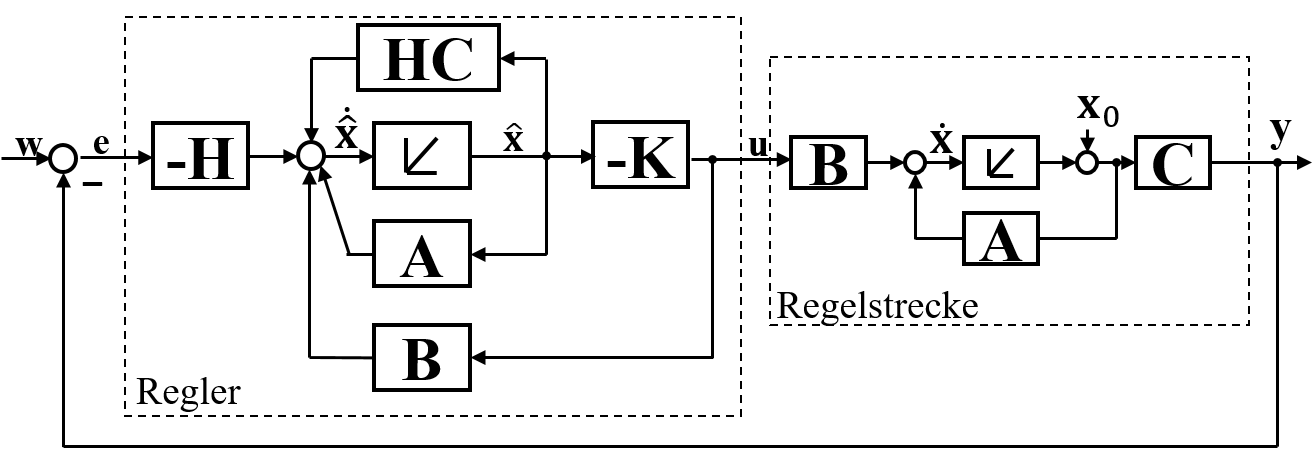
\includegraphics[width=0.4\linewidth]{bilder/observer_alternativ}
\end{center}
\begin{itemize}
	\item Dabei gelten die Gleichungen
	\item[] $\dot{\hat{x}} = \left( \boldsymbol{A}-\boldsymbol{BK}-\boldsymbol{HC}\right)\hat{x}-\boldsymbol{H}e$
	\item[] $u = -\boldsymbol{K}\hat{x}$
	\begin{itemize}
		\item Natürlich kann $e$ auch mit $w,\boldsymbol{A},\boldsymbol{B},\boldsymbol{C},\boldsymbol{K}$ ausgedrückt werden.
	\end{itemize}
	\item Für den Open-Loop ($w=0$) gilt:
	\item [] $G_o(s) = \boldsymbol{K}\left( s\boldsymbol{I}-\boldsymbol{A}+\boldsymbol{BK}+\boldsymbol{HC}\right)^{-1}\boldsymbol{H} \cdot\boldsymbol{C}\left(s\boldsymbol{I}-\boldsymbol{A}\right)^{-1}\boldsymbol{B}$
	\item Die Transferfuntktion des Reglers ist
	\item[] $G(s) = \frac{U(s)}{E(s)} = 
	\boldsymbol{K}\left( s\boldsymbol{I}-\boldsymbol{A}+\boldsymbol{BK}+\boldsymbol{HC}\right)^{-1}\boldsymbol{H}$
\end{itemize}

\subsection{LQG}
\begin{itemize}
	\item [1.] $\boldsymbol{AP}+\boldsymbol{PA}^T-\boldsymbol{PC}^T\boldsymbol{CP} ~~=-\rho\boldsymbol{BB}^T ~~=-\boldsymbol{Q}$
	\begin{itemize}
		\item Positiv definite Lösung von $\boldsymbol{P}$ wählen
	\end{itemize}
	\item [2.] $\boldsymbol{H} =\boldsymbol{PC}^T$
	\item Grosse Werte für $\rho ~~\Rightarrow$ Grosses Prozessrauschen führt zu grosser Verstärkung durch den Beobachter. Daher ist dieser anfälliger für verrauschte Signale.
\end{itemize}

\subsection{LTR (Loop transfer recovery)} 
\begin{itemize}
	\item LTR befasst sich mit der Platzierung der Pole von Regler und Beobachter, mit dem Ziel eine ausreichende Phasen- und Amplitudenreserve zu erreichen
	\item Die Phasen Reserve der einzelnen Teilsysteme ist min $\pm$\ang{60} und die Amplitudenreserve $\in \left[0.5\right. \ldots \infty \left.\right[$
	\item Das zusammengesetzte System hat jedoch \underline{keine} garantiert Reserve (weder Amplituden- noch Phasenreserve)
	\item Wird ein LQR (Regler) mit den Gewichtungsmatrizen ausgerechnet, erhalten wir die K-Matrix
	\item Wird ein LQG (Beobachter) mit den Gewichtungsmatrizen ausgerechnet, erhalten wir die H-Matrix
	\item Die H-Matrix wird entsprechnd der K-Matrix berechnet, wobei die Gewichtungen 
	\begin{itemize}
		\item $\boldsymbol{Q} = \rho \boldsymbol{BB}^T$ wobei $\boldsymbol{Q}$ das Prozessrauschen darstellt
		\item $\boldsymbol{R} = \boldsymbol{I}$ wobei $\boldsymbol{R}$ das Sensorrauschen darstellt
		\item Wenn R klein wird, wird Q gross und umgekehrt
	\end{itemize} 
	\item Bei einem minimalphasigen System gilt
	\item[] $\lim\limits_{\rho\rightarrow \infty}\left(G_o(s)\right) = \boldsymbol{K}\left(s\boldsymbol{I}-\boldsymbol{A}\right)^{-1}\boldsymbol{B}$
\end{itemize}

\subsubsection{Anwendung von LTR mit LQR und LQG}
\begin{itemize}
	\item Möglichkeit zum Erreichen der Reserve, wenn entweder der Regler oder der Beobachter beliebig gewichtet werden soll
\end{itemize}




\begin{tabularx}{\linewidth}{rp{.1\linewidth} rp{.1\linewidth}}
	\textbf{LQR beliebig}		&		&							\hspace{2.5cm} \textbf{LQG beliebig}& \\				
	Wert für LQR	&beliebig 										& 	Wert für LQR	&$\boldsymbol{Q} = \rho\boldsymbol{C}^T\boldsymbol{C}$\\
	Wert für LQG	&$\boldsymbol{Q} = \rho\boldsymbol{BB}$			& &	$\boldsymbol{R} = \boldsymbol{I}$ \\
					&$\boldsymbol{R} = \boldsymbol{I}$				& &	$\rho \ge 0$\\
					&$\rho \ge 0$									&Wert für LQG &beliebig	
\end{tabularx}
\newpage
\section{Systemidentifikation}
\subsection{Basics}
\begin{itemize}
	\item Gewinnen von Informationen über ein nur teilweises oder ganz unbekanntes System
	\item \textbf{Achtung:} Bei Bode-Diagramm ist X-Achse in $\omega$ und nicht in der Frequenz 
	\begin{itemize}
		\item Reminder: $x \left[db\right] = 20\log_{10}\left(x\right)$
	\end{itemize}
	\item Erstellen von mathematischen Modellen basierend auf den Messergebnissen
	\item 
\end{itemize}

\subsection{Nicht Parametrische Identifikation}
\begin{itemize}
	\item Anregung eines Systems mit dem Sinus einer einzelnen Frequenz und beobachten des Ausganges
	\item Beobachten der Antwort und entsprechende Erstellung des Bode-Diagramms
	\item Für eine Totzeit ($e^{-st_t}$) geht der Phasengang mit zunehmender Frequenz zu $-\infty$, der Amplitudengang wird nicht beeinflusst. 
\end{itemize}
\begin{figure}[h!]
	\centering
	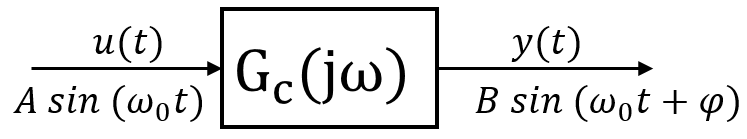
\includegraphics[width=0.25\linewidth]{bilder/sysIdent1}
\end{figure}

\subsubsection{Bode $\Leftrightarrow$ Übertragungsfunktion}
\begin{tabularx}{\linewidth}{p{0.25\linewidth} p{0.25\linewidth} p{0.25\linewidth} p{0.25\linewidth} }
	\textbf{Integrator} 	&\textbf{Tiefpass}			&\textbf{Hochpass}				&\textbf{Resonanz}	\\
	%Zeile 2 mit Allen Bildern
	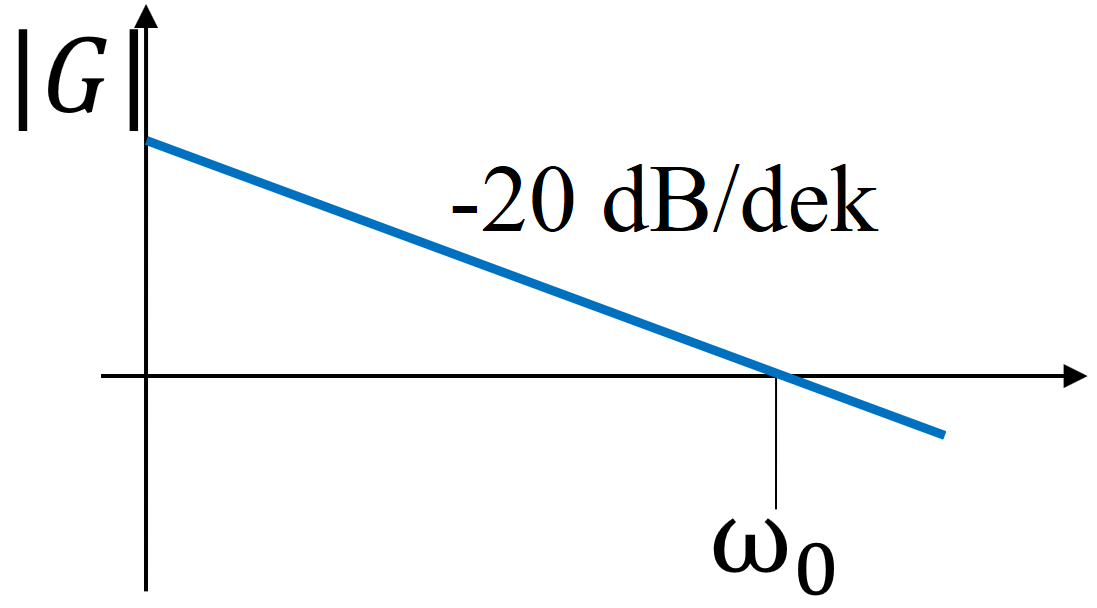
\includegraphics[width=.75\linewidth]{bilder/sysIdentInt}&
	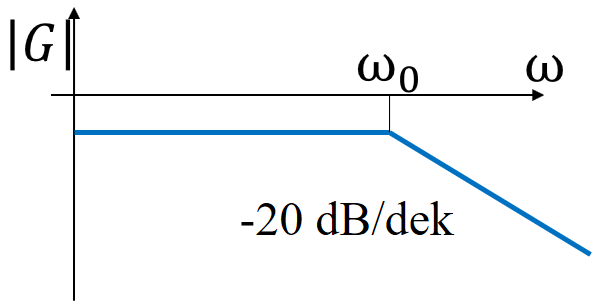
\includegraphics[width=.75\linewidth]{bilder/sysIdentTiefpass}&
	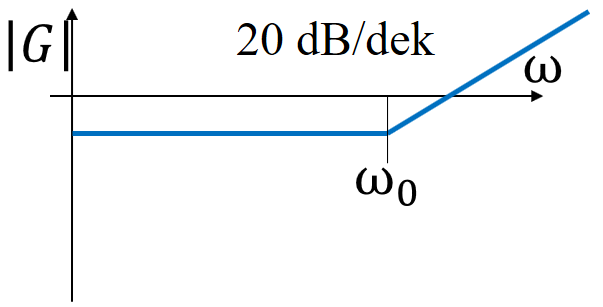
\includegraphics[width=.75\linewidth]{bilder/sysIdentHochpass}&
	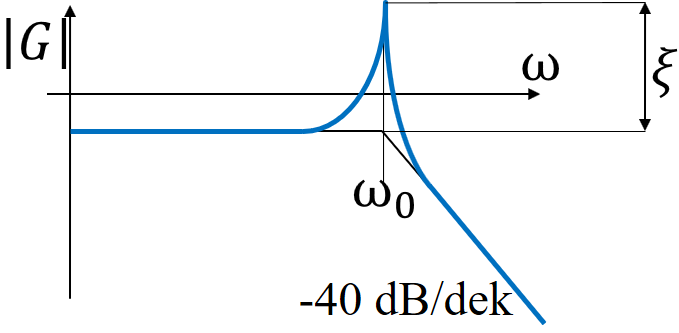
\includegraphics[width=.75\linewidth]{bilder/sysIdentResonanz}\\
	%Zeile 3 Mit den Formeln
	\begin{equation*}
		G\left(s\right) = \frac{\omega_0}{s}
	\end{equation*}&
	\begin{align*}
		G\left(s\right)= \frac{1}{\frac{1}{\omega_0}s+1}  \\
						=\frac{\omega_0}{s+\omega_0}
	\end{align*}&
	\begin{equation*}
		G\left(s\right)=\frac{1}{\omega_0}+1
	\end{equation*}&
	\begin{align*}
	\nonumber
		G\left(s\right) =\frac{1}{s^2T_0^2+2\xi T_0+1} \\
		T = \frac{2\pi}{\omega_0}
	\end{align*} 
\end{tabularx}

\subsubsection{Leakage-Effekt}
\begin{itemize}
	\item Zu erkennen wenn:
	\begin{itemize}
		\item Verstärkung zwischen $u(s)$ und $y(s)$ auf einmal fast konstant bei 0 dB bleibt 
		\item Das bekannte und gleichzeitig gemessene Eingangssignal $u(s)$ scheint bei zunehmender Frequenz gedämpft zu sein. 
		\item Ein untypischer Knick, der in dem Bode-Diagramm auftritt. Hierbei muss sichergestellt werden, dass dieser nicht aufgrund der Regelstrecke ist
	\end{itemize}
	\item In untenstehenden Grafiken sind Beispiele von Leakage-Effekten gezeigt. Die feine Linie ist dabei das wahre Verhalten des Systems, die dicke Linie das gemessene Verhalten des Systems.
\end{itemize}
\begin{figure}[!ht]
	\centering
	\subfloat[Gemessene Amplitude von $u(s)$ und $y(s)$ \label{subfig:Leakage1}]{
		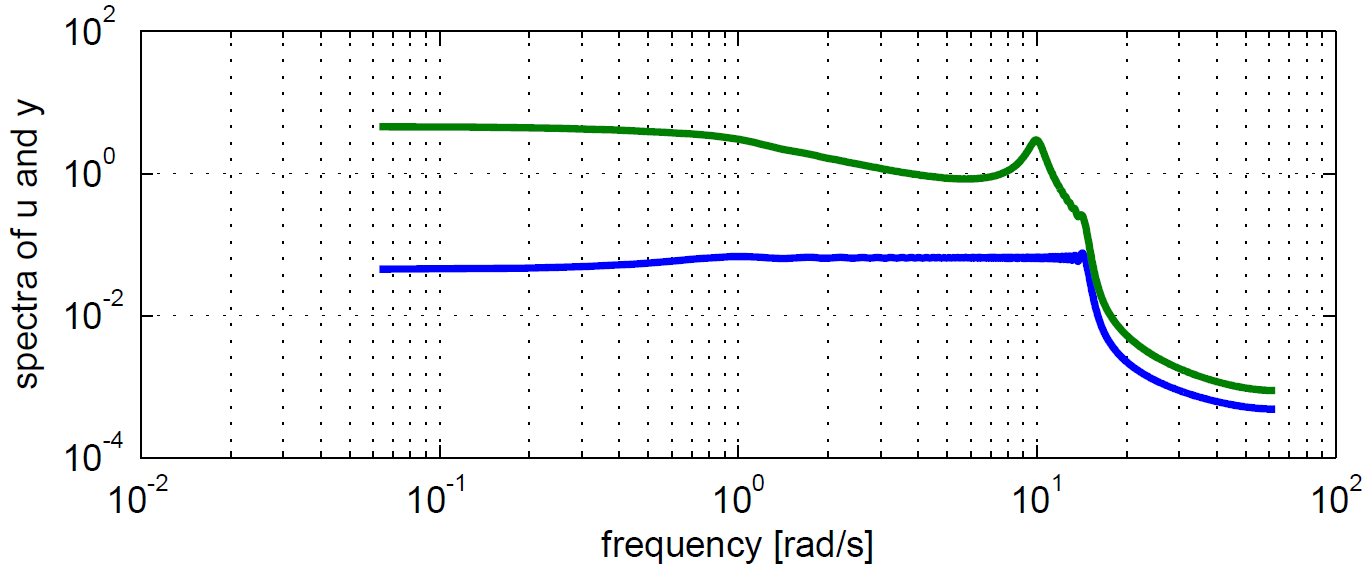
\includegraphics[width=0.3\textwidth]{./bilder/LeakageEffect1.PNG}
	}
	\subfloat[Amplitudengang der Regelstrecke \label{subfig:Leakage2}]{
		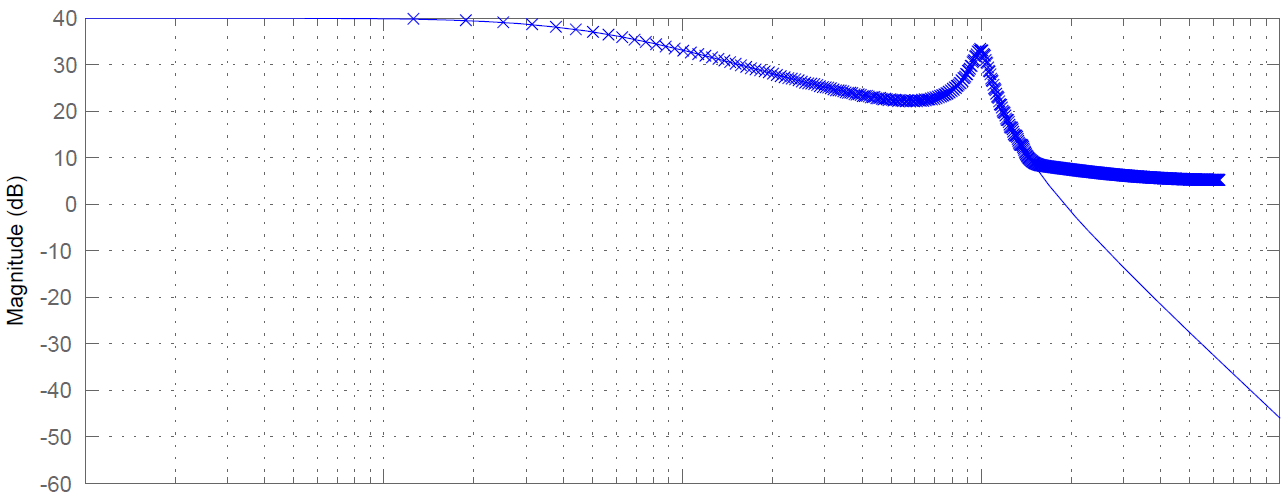
\includegraphics[width=0.3\textwidth]{./bilder/LeakageEffect2.PNG}
	}
	\subfloat[Phasengang der Regelstrecke \label{subfig:Leakage3}]{
		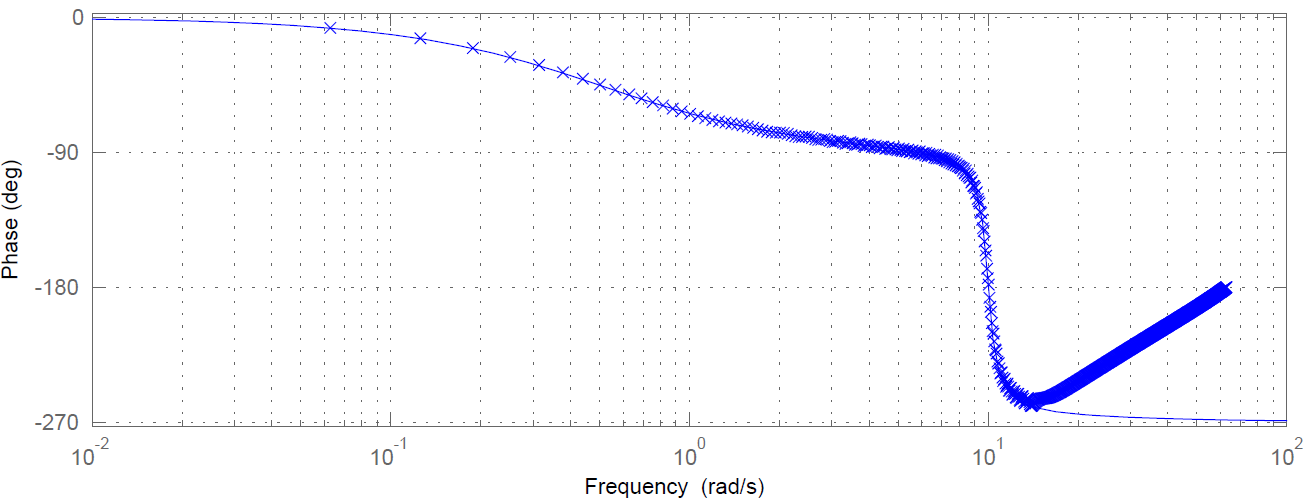
\includegraphics[width=0.3\textwidth]{./bilder/LeakageEffect3.PNG}
	}\\
	\textit{Quelle: Kottmann, Markus (2012): Advanced Control. Introduction to System Idenfication. Version 1.3. 13}
	\label{fig:Leakage}
\end{figure}

\subsubsection{Schrittantwort}
\begin{itemize}
	\item Gibt meist kein ausreichend genaues Modell für die Regelung
	\item Einige Dinge können dennoch mit der Schrittantwort charakterisiert werden, nämlich:
	\begin{itemize}
		\item Statische Verstärkung (DC-Gain)
		\item Dominante Zeitkonstante
		\item Totzeit
		\item Ob das System Resonanzen hat
		\item Minimalphasigkeit des Systems
	\end{itemize}
	\item Schwingt die Schrittantwort zuerst in das Negative, hat das System eine Nullstelle in der rechten Halbebene
	\begin{itemize}
		\item System ist nicht minimalphasig
	\end{itemize}
\end{itemize}

\begin{tabularx}{\linewidth}{p{0.32\linewidth} p{0.32\linewidth} p{0.32\linewidth}}
	\textbf{Nicht minimalphasig}			&\textbf{Totzeit}				&\textbf{PT2}		\\
	%Zeile 2 mit Allen Bildern
	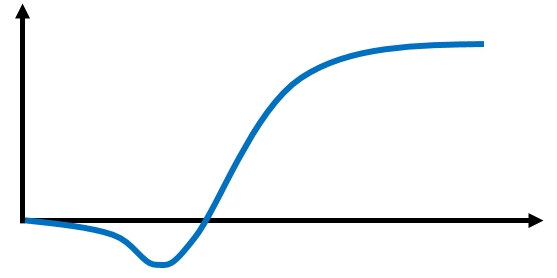
\includegraphics[width=.75\linewidth]{bilder/step1.png}&
	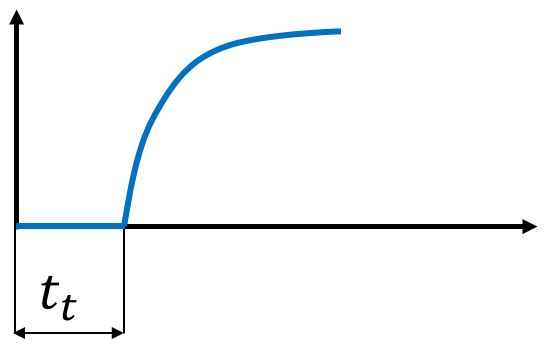
\includegraphics[width=.75\linewidth]{bilder/step2.png}&
	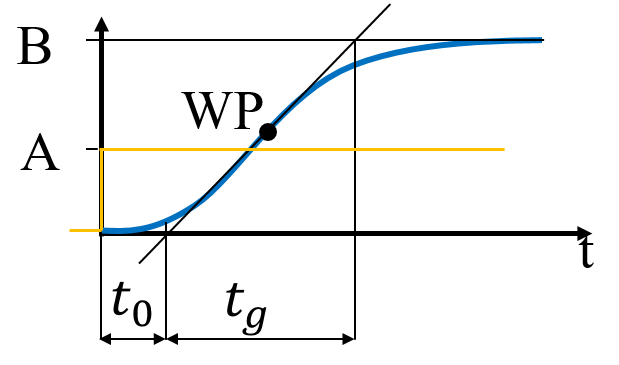
\includegraphics[width=.75\linewidth]{bilder/step3.png} \\
	%Zeile 3 Mit den Formeln
	& \begin{align*}
		G(s)_\text{Totzeit} = e^{-st_t}\\
		G(z)_\text{Totzeit} = z^(-1)
	\end{align*} 
	& \begin{equation*}
	G(s) = \frac{B}{A}\cdot e^{\frac{-s}{T_0}}\cdot \frac{1}{sT_g+1}
	\end{equation*}
\end{tabularx}

\subsection{Parametrische Identifikation}
\begin{itemize}
	\item Identifizieren von Systemen deren Strukturen bekannt sind
	\item Wenn keine Spezielle Form der Systembeschreibung gewählt wird, sind $(n+1)^2$ Parameter zu ermitteln (Matrizen A,B,C,D)
	\begin{itemize}
		\item  Wenn eine spezifische Form gewählt wird (z.B. Regelnormalform) sind es nur noch $2n+1$ Parameter
	\end{itemize}
	\item [1.] Die Matrizen des Systems herleiten (mit den Variablen des Systems, so z.B. Federkonstanten, Dämpfungen, etc.). 
	\item [2.] $G(s)$ aus den Matrizen bestimmen
	\item [3.] Messungen vornehmen und mit den Messergebnissen z.B. Überkoeffizientenvergleich mit $G(s)$ Werte der Parameter bestimmen
\end{itemize}

\subsection{LS-Verfahren}
\begin{itemize}
	\item Fitten von Daten
	\item Es gilt: $N$: Die Anzahl der Datensätze, $n$: Die Anzahl der Variablen
	\item LS zielt darauf ab den Fehler zu minimieren
	\item Verfahren funktioniert besonders gut, wenn gesuchte Funktion Linear in Parameter (im Beispiel $\theta$) ist.
	\begin{itemize}
		\item[] $y_j = f(u_j) = u_j\theta_1+u^2_j\theta_2+\ldots+u^n\theta_n$
		\item $y_j$: Gemessenes Signal, \quad $u_j$: Eingangssignal, \quad $\theta_j$: Parameter
	\end{itemize}
	\item Beispiel (\textit{Quelle: Kottmann, Markus (2012): Advanced Control. Introduction to System Idenfication. Version 1.3. 21}):
	\begin{itemize}
		\item Wenn System überbestimmt ist, braucht es den Fehlerterm $\varepsilon$
		\item Ziel ist es die Kostenfunktion  $J= \vert\varepsilon\vert^2$ klein zu halten (somit also auch $\varepsilon$ klein zu halten)
		\item Mit der gezeigten Formel für $\theta$, wird das $\varepsilon$ bereits minimiert!
	\end{itemize}
\end{itemize}
\begin{align*}
	1. &= 0.8 \theta_1 + 0.8^2\theta_2 = 0.8 \theta_1+0.64\theta_2\\
	2.5 &= 2 \theta_1 + 2^2\theta_2 = 2\theta_1+4\theta_2\\
	2 &= 3 \theta_1 + 3^2\theta_2 = 3 \theta_1+9\theta_2\\
 	\underbrace{ \begin{bmatrix}
 	1 \\ 2.5\\2
 	\end{bmatrix}}_y &= 
	\underbrace{\begin{bmatrix}
		0.8 	& 	0.64\\
		2   	&	4	\\
		3		&	9
		\end{bmatrix}}_\Phi
	\underbrace{\begin{bmatrix}
		\theta_1\\
		\theta_2
		\end{bmatrix}}_\theta\\
	y &= \Phi\theta+\varepsilon\\
	\theta &= \left(\Phi^T\Phi\right)^{-1}\Phi^Ty
\end{align*}

\subsubsection{LS-Verfahren für Zeitdiskrete Systeme}
\begin{itemize}
	\item Vorgehen:
	\begin{itemize}
		\item $G(z)$ umformen, sodass Nenner ein Summand ohne $z$ hat
		\item []$G(z) = \frac{Y(z)}{X(z)} \Leftrightarrow Y(z) = G(z)U(z)$
		\item Parameter (z.B. $a$ und $b$) sind in $G(z)$ enthalten $\Rightarrow$ das ist der Vektor $\theta$
		\item []$  az^{-i}\cdot u(z) \Leftrightarrow au(k-i)$
		\item Umstellen, dass $y(k)$ als Funktion von $y(k-i)$ und $x(k-i)$
		\item $u(k-i)$ und $y(k-i)$ sind die Messwerte am Eingang resp. Ausgang, Versetzt um $i$ Zeitschritte
		\item Daraus erstellen der Matrix $\Phi$ und des Vektors $y$ 
		\item Jeweils eine Zeile je möglicher Gleichung
	\end{itemize}
	\item Siehe auch Kapitel \ref{subsec:LSDynSys}, dort ist die Formel für mehrere Gleichungen angewendet
	\item Minimalbeispiel
\end{itemize}
\begin{align*}
	G(z) &= \frac{Y(z)}{X(z)} = \frac{a}{z\cdot(z+b)}\\
	G(z) &= \frac{az^{-2}}{1+bz^{-1}}\\
	Y(z)\cdot \left(1+bz^{-1}\right) &= X(z)\cdot \left(az^{-2}\right)\\
	Y(z) &= az^{-2}X(z)-bz^{-1}Y(z)\\
	y(k) &= ax(k-2)-by(k-1)\\
	y(k) &= \begin{bmatrix}
		x(k-2) & -y(k-1)
	\end{bmatrix}\begin{bmatrix}
	a \\b
	\end{bmatrix}
\end{align*}

\subsubsection{LS-Verfahren bei Problemen mit Bode-Diagrammen}
\begin{itemize}
	\item Im Komplexen Raum betrachten
	\begin{itemize}
		\item von Amplitudengang und Phasenwinkel zu Polarform
		\item $\vert G(j\omega)\vert=A\left[\text{dB}\right]$ und $\angle G(j\omega) = \varphi \left[\si{\degree}\right] \quad \Rightarrow 10^{A/20}\cdot e^{j\varphi/180}$ 
	\end{itemize}
	\item Minimalbeispiel mit Resonanz und DC-Verstärkung (Gl. = Kommentar zu Gleichung im nachfolgenden Beispiel)
	 \begin{itemize}
	 	\item [Gl.\ref{eq:LS1}:] Normieren, dass Nennerpolynom mit  $s^i$ beginnt
	 	\item [Gl.\ref{eq:LS2}:] Auflösen nach $G(s)s^i$
	 	\item [Gl.\ref{eq:LS3}:] In Frequenzraum wechseln $s\Leftrightarrow(j\omega)$
	 	\item [Gl.\ref{eq:LS4}:] In Matrizen Form bringen (eine Zeile je erhaltenen Messpunkt)
\begin{itemize}
	 	 	\item Nun Werte Einsetzen, dabei wie oben beschrieben Informationen von Bode-Diagramm in Polarform bringen und einsetzen für $G(j\omega)$ 
	 		\item $(j\omega)$ ist $j$ Multpliziert mit der Frequenz an welcher der Messpunkt aufgenommen wurde
\end{itemize}
	 	\item [Gl.\ref{eq:LS5}:] $\tilde{\Phi}$ und $\tilde{y}$ aus dem Real- und Imaginäranteil bilden (Zeilenzahl verdoppelt sich)
	 	\item [Gl.\ref{eq:LS6}:] LS-verfahren so, dass alle Werte am besten gefittet werden. 
	 \end{itemize}
\end{itemize}
\begin{align}
	\label{eq:LS1}
	G(s) &= \frac{k\omega^2}{s^2+2\xi\omega s+\omega^2}\\
	\label{eq:LS2}
	G(s)s^2&=k\omega^2-2G(s)\xi\omega s-G(s)\omega^2\\
	\label{eq:LS3}
	G(j\omega)\left(j\omega\right)^2 &= k\omega^2-2G(j\omega)\xi\omega(j\omega) - G(j\omega)\omega^2\\
	\label{eq:LS4}
	\underbrace{\begin{bmatrix}
		G(j\omega)\left(j\omega\right)^2 
	\end{bmatrix}}_y	&=\underbrace{\begin{bmatrix}
		1	&	-2G(j\omega)(j\omega)	&	-G(j\omega)
	\end{bmatrix}}_\Phi	
	\underbrace{\begin{bmatrix}
		k\omega^2\\
		\xi\omega\\
		\omega^2
	\end{bmatrix}}_\theta\\
	\label{eq:LS5}
	\tilde{y} &= \begin{bmatrix}
		\text{Re}\left(y\right)\\
		\text{Im}\left(y\right)
	\end{bmatrix}	\qquad 
		\tilde{\Phi} = 
	\begin{bmatrix}
		\text{Re}\left(\Phi\right)\\
		\text{Im}\left(\Phi\right)
	\end{bmatrix}\\
	\tilde{y} &= \tilde{\Phi}\theta+\varepsilon\\	
	\label{eq:LS6}
	\theta &= \left(\tilde{\Phi}^T\tilde{\Phi}\right)^{-1}\tilde{\Phi}^T\tilde{y}
\end{align}


\subsubsection{Gewichtetes LS-Verfahren}
\begin{itemize}
	\item Gleichungen haben unterschiedliche Gewichtung (z.B. Arbeitspunkt höher gewichten)
	\begin{itemize}
		\item Gewichtung mit Faktor $\lambda$
		\item Da Gewichtungsmatrix immer als $L^TL$ erscheint, muss für Faktor $\lambda$ stattdessen$\sqrt{\lambda}$ genommen werden
	\end{itemize}
	\item Angewendet auf obige Gleichung ergibt die Auflösung nach $\theta$: 
\end{itemize}
\begin{align*}
	L &= \begin{bmatrix}
		\sqrt{\lambda_1}&0					&\ldots&0\\
		0				&\sqrt{\lambda_2}	&\ldots&0\\
		\vdots			&\vdots				&\ddots&0\\
		0				&0					&\ldots&\sqrt{\lambda_n	}	
	\end{bmatrix}\\
	\theta &= \left(\Phi^TL^TL\Phi\right)^{-1}\Phi^TL^TLy
\end{align*}

\subsubsection{Markov-Annahme unter Verwendung der Co-varianz-Matrix}
\begin{itemize}
	\item $\varepsilon$ ist in Gaussverteilung und der Erwartungswert liegt bei 0
	\item Dann ist die Co-Varianzmatrix: $V= \varepsilon\varepsilon^T$
	\item $\varepsilon$ ist Abweichung zwischen mit dem LS-Verfahren erhaltenem Modell und dem effektiven Messwert
	\item Dann kann für die Gewichtungsfunktion $L^TL=V^{-1}$ genommen werden.
\end{itemize}

\subsection{LS-Verfahren für dynamische Systeme}
\label{subsec:LSDynSys}
\begin{itemize}
	\item Ziel: Ein System welches in Bewegung ist durch zwei Polynome abzubilden
	\item $\varepsilon$ soll möglichst 0 werden
	\item Zwei verschiedene Darstellungsmöglichkeiten für die Modelle (Ausgangsfehlermodell: \ref{subfig:LSNormal}, ARX-Modell: \ref{subfig:LSARX})
\end{itemize}
\begin{figure}[!h]
	\centering
	\subfloat[Ausgangsfehlermodell \label{subfig:LSNormal}]{
		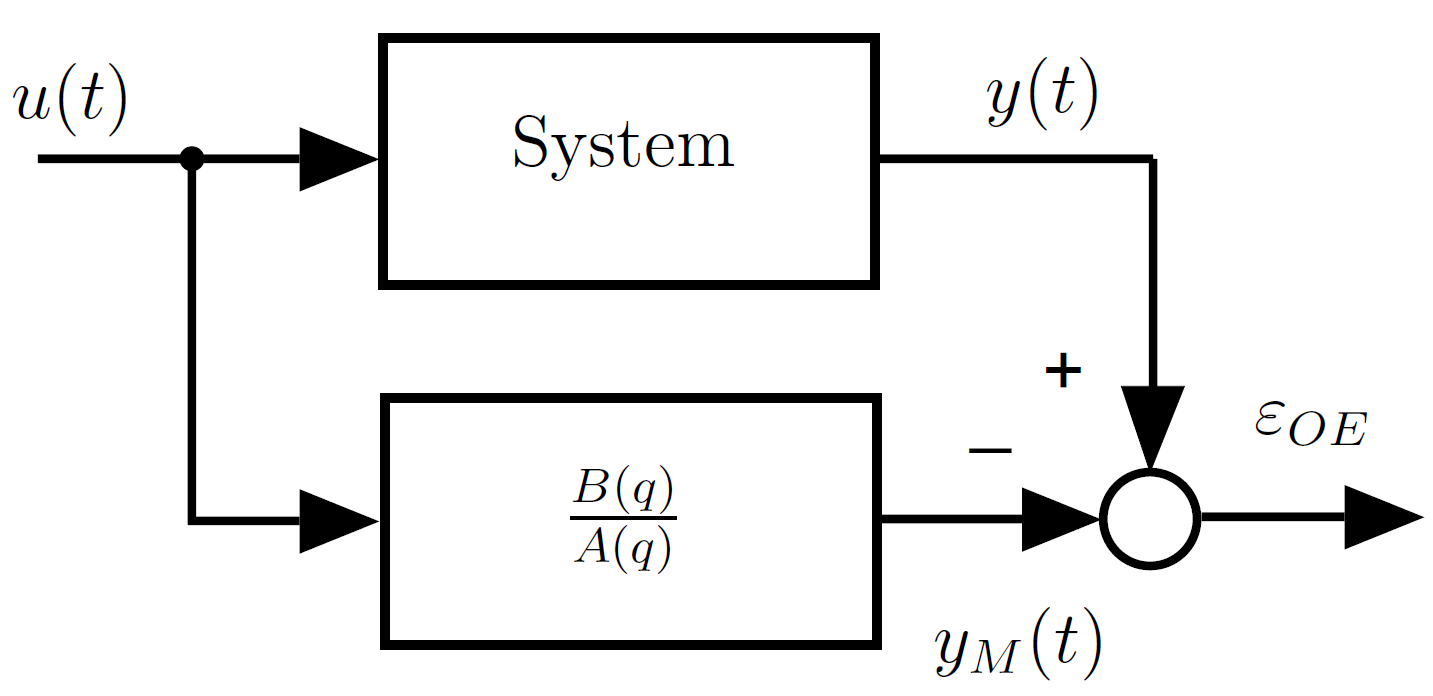
\includegraphics[width=0.3\textwidth]{./bilder/LSNormal.PNG}
	}\hspace{0.1\linewidth} 
	\subfloat[ARX-Modell \label{subfig:LSARX}]{
		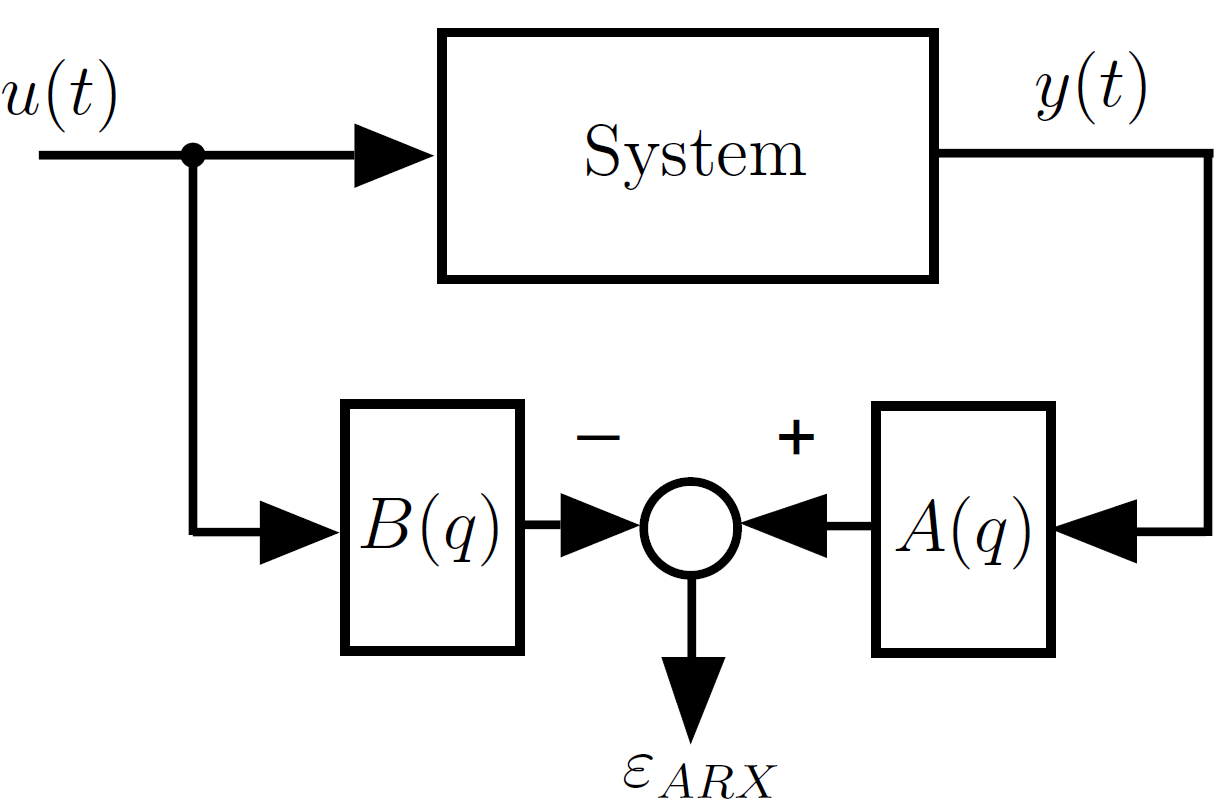
\includegraphics[width=0.25\textwidth]{./bilder/LSARX.PNG}
	}\\
	\caption{Zwei Darstellungsmöglichkeiten für Modelle welche ein LS-Verfahren für dynamische Systeme ermöglichen}
	\textit{Quelle: Kottmann, Markus (2012): Advanced Control. Introduction to System Idenfication. Version 1.3. 26}
	\label{fig:LS}
\end{figure}

\begin{itemize}
	\item Mit der ARX-Struktur kann $y(t)$ angesehn werden als:
	\begin{itemize}
		\item $y(t)$ ist hierbei eine Messung zum Zeitpunkt $k$ und setzt sich aus den vorherigen diskreten Messungen und Eingangssignalen zusammen
	\end{itemize}
\end{itemize}
\begin{align*}
	y(k) 	&= -a_1y(k-1)-\ldots -a_ny(k-n)+b_1u(k-1)+\ldots b_mu(k-m)+\varepsilon(k)\\
			&= \begin{pmatrix}
				-y(k-1) &\ldots &-y(k-n) & u(k-1) & \ldots & u(k-m)
			\end{pmatrix}
			\begin{pmatrix}
				a_1\\ 
				\vdots \\
				a_n\\
				b_1\\
				\vdots\\
				b_m
			\end{pmatrix}+\varepsilon(k)
\end{align*}
\begin{itemize}
	\item Wenn nun $N$ Messungen gemacht werden (somit sind es $0\ldots N$ Messungen)
	\item $\Phi$ sind dabei die am Eingang ($u(k)$ und am Ausgang($y(k)$) gemessenen Signale
	\item Es muss solang gemssen werden, bis $\text{rank}(\Phi) \leq n+m$ (n = Anz. Ausgangssignale, m = Anz. Eingangssignale)
	\item Rekursives LS-Verfahren, siehe Skript s.29
\end{itemize}
\begin{align*}
	\underbrace{\begin{pmatrix}
		y(0)\\
		\vdots\\
		y(N)
	\end{pmatrix}}_y
			&= \underbrace{\begin{pmatrix}
					-y(-1) 	&\ldots 	&-y(-n) 	& u(-1)   	&\ldots 	& u(-m)\\
					\vdots	&\ddots		&\vdots		&\vdots		&\ddots		&\vdots\\	
					-y(N-1) &\ldots 	&-y(N-n) 	& u(N-1) 	&\ldots 	& u(N-m)
					\end{pmatrix}}_{\Phi = \text{Messwerte von Ein- und Ausgnag}}
				\underbrace{\begin{pmatrix}
					a_1\\ 
					\vdots \\
					a_n\\
					b_1\\
					\vdots\\
					b_m
				\end{pmatrix}}_\theta+
				\underbrace{\begin{pmatrix}
					\varepsilon(0)\\
					\vdots\\
					\varepsilon(N)
				\end{pmatrix}}_\varepsilon\\
	\theta	&= \left(\Phi^T\Phi\right)^{-1}\Phi^Ty
\end{align*}
\newpage
\section{Diskretisierung und Implementierung}
\subsection{Basics}
\begin{figure}[h!]
	\begin{minipage}{0.5\linewidth}
		\centering
		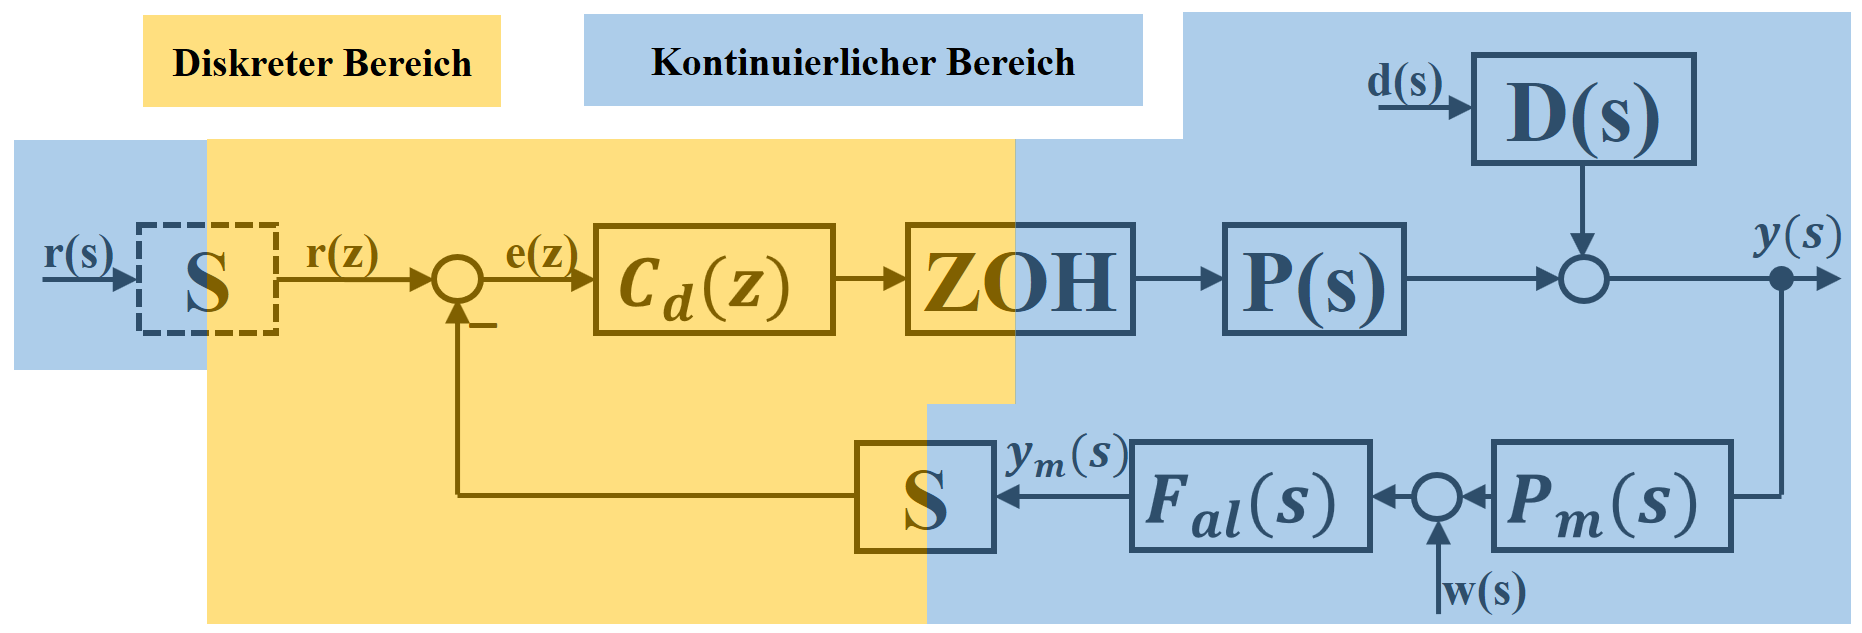
\includegraphics[width=.9\linewidth]{bilder/DiskretesSystem}
		\label{fig:diskretessystem}
	\end{minipage}
	\begin{minipage}{0.45\linewidth}
		\footnotesize
		\begin{tabular}{rl}
			S 						&= Samplingmodul (ADC)\\
			ZOH 					&= Zero Order Hold (DAC)\\
			P(s)					&= Regelstrecke\\
			$\text{C}_d$			&= diskreter Regler\\
			$\text{F}_{al}$			&= anti aliasing Filter\\
			$\text{P}_m$			&= Sensorübertragungsfunktion\\
			w						&= Noise Signal zum Sensor\\
			$\text{P}_m+\text{w}$	&= Sensor Modell\\
			d						&= Noise von der Regelstrecke\\
			D						&= Shaping Filter
		\end{tabular}
	\end{minipage}
\end{figure}
\begin{itemize}
	\item Hier ist nicht mehr linke Halbebene ausschlaggebend über stabilität, sondern ob alle Pol- und Nullstellen innerhalb des Einheitskreises liegen
\end{itemize}

\subsection{Diskretisierung von Reglern}
\begin{itemize}
	\item In Zeitdomain $\dot{y}(t) $ wird in Laplace-Raum zu $sy(s)$ in diskretisierten Raum entspricht dies $\dot{y(t)}\sim\frac{y(kt)-y(kt+T)}{T}$
	\item Die Bildung der Differenzengleichung erfolgt mit $C(z) = \frac{y(z)}{e(z)}$
\end{itemize}
\subsubsection{Diskretisierungsmethoden}
\begin{itemize}
	\item Entsprechend in der Übertragungsfunktion alle $s$ mit dem entsprechenden Term der Transformation ersetzten. Dabei ist $T$ die Abtastzeit
	\item Die Bilineare Transformation bildet die linke halbebene in den Einheitskreis ab. (siehe Abbildung \ref{fig:Tustin})
	\begin{itemize}
		\item Somit ist garantiert, dass stabile Regler auch im diskreten stabil bleiben.
	\end{itemize}
	\item Pole-Zero-Matching: Wenn der Regler unendlich Nullstellen hat, können diskrete Pole bei -1 angenommen werden
\end{itemize}
\begin{align*}
	\text{\textbf{Vorwärtseuler}} \qquad & s=\frac{z-1}{T}\\
	\text{\textbf{Rückwärtseuler}} \qquad & s=\frac{z-1}{Tz}\\
	\text{\textbf{Tustin / Bilinear}} \qquad & s=\frac{2}{T}\frac{z-1}{z+1}\\
	\text{\textbf{Zero-Order-Hold}} \qquad& G(z) = \frac{z-1}{z}\mathcal{Z}\left\{\mathcal{L}^{-1}\left\{\frac{G(s)}{s}\right\}\right\}\\
	\text{\textbf{Pole and zero Matching}} \qquad & z=e^{s\cdot T}
\end{align*}
\begin{figure}[h!]
	\centering
	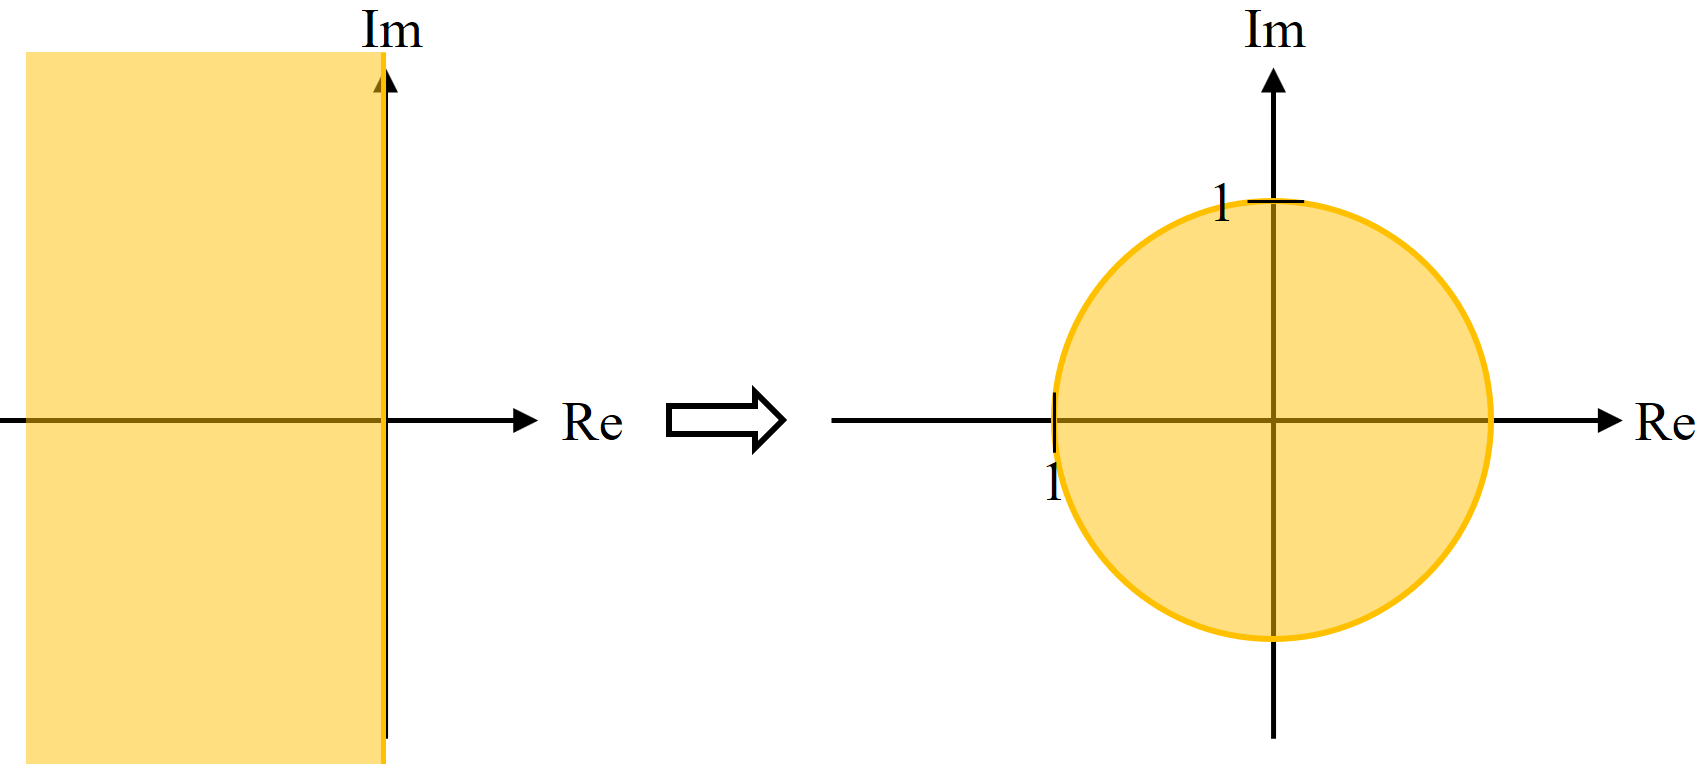
\includegraphics[width=0.3\linewidth]{bilder/Tustin}
	\caption{Tustin-Verfahren führt linke Halbebene in Einheitskreis über}
	\label{fig:Tustin}
\end{figure}

\subsubsection{Wahl der Sampling Time}
\begin{itemize}
	\item Gründe für Maximierung der sampling Time
	\begin{itemize}
		\item Pole entfernen sich von 1, somit wird controllaw nummerisch stabiler. (weniger anfällig für Quantisierungsfehler)
		\item Hardware muss weniger leistungsfähig sein $\Rightarrow$ günstiger
		\item Differenzierende Regler funktionieren besser (Glättung des Signals, da Ableitung über längere Zeitperiode)
	\end{itemize}
	\item Gründe für Minimierung der sampling Time
	\begin{itemize}
		\item Wenn A/D und D/A wandler synchronisiert sind, führt dies zu einer kleineren Totzeit
		\item Bei Verwendung eines Anti-Aliasing-Filters (für verrauschte Signale) ist der Phasenverlust kleiner
		\item Je kleiner die Sampling Time, desto weniger Phasenverlust durch das ZOH-Glied
	\end{itemize}
	\item Maximale Frequenz: Signal darf keine Frequenzen enthalten die grösser sind als halbe Abtastfrequenz
	\begin{itemize}
		\item [] $f_\text{max}\leq \frac{1}{2}\cdot f_\text{Abtast}$
		\item Kann hergeleitet werden mit Shannon-Nyquist
	\end{itemize}
	\item Das Shannon-Sampling Theorem besagt: Sampling Frequenz (in rad) soll grösser sein als $20\omega_d$ des offenen Regelkreises ($\omega_d$ = Durchtrittsfrequenz)
\end{itemize}

\subsection{Windup und weitere Gefahren}
\begin{itemize}
	\item Regler summiert Fehler zu schnell auf (da Regelstrecke langsam und Abtastzeit hoch ist)
	\item Wenn zwei Pole bei einem digitalen Regler zu nahe zusammen liegen, muss mit Quantisierungsproblemen gerechnet werden. 
\end{itemize}
\newpage
\section{H$\infty$-Regler}
\begin{itemize}
	\item Wenn die Regelstrecke nicht exakt bekannt ist, oder sich mit der Zeit verändern kann
	\item Kompensieren einer Abweichung zum theoretisch entworfenem Regler
	\begin{itemize}
		\item Dabei stellt $\Delta$ die Abweichung zur theoretisch ermittelten Strecke dar. 
		\item Eine andere Bezeichnung für $\Delta$ ist Modellunsicherheit
	\end{itemize}
	\item $P_0$ bezeichnet die nominale Regelstrecke
\end{itemize}
\begin{figure}[h!]
	\centering
	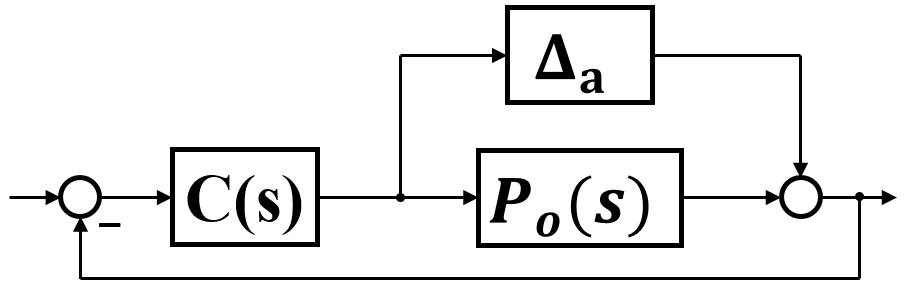
\includegraphics[width=0.25\linewidth]{bilder/HInf1}
	\label{fig:hinf1}
\end{figure}

\subsection{Basics}
\begin{itemize}
	\item Die H$\infty$-Norm ist der höchste Punkt im Bode-Diagramm der zu untersuchenden Funktion
	\item $\text{H}_\infty\text{-Norm} = \lVert P(s) \rVert_\infty$
	\begin{itemize}
		\item In untenstehender Abbildung ist ein Beispiel gezeigt. Die $\text{H}_\infty\text{-Norm}$ ist für diese Funktion $A$
	\end{itemize}
	\item Die Robuste Regelung funktioniert bei den klassischen Stabilitätsbeobachtung (Phasen- und Amplitudenreserve)
	\begin{itemize}
		\item Es gibt keine analytische Optimierungsmethode
		\item Auch bei scheinbarer Stabilität (durch übliche Kriterien) ist diese keine Garantie für Stabilität des Regelkreise. 
	\end{itemize}
\end{itemize}

\begin{figure}[!ht]
	\centering
	\subfloat[$\text{A}=\lVert H \rVert_\infty$ von $G(s)$ \label{subfig:hinf1}]{
		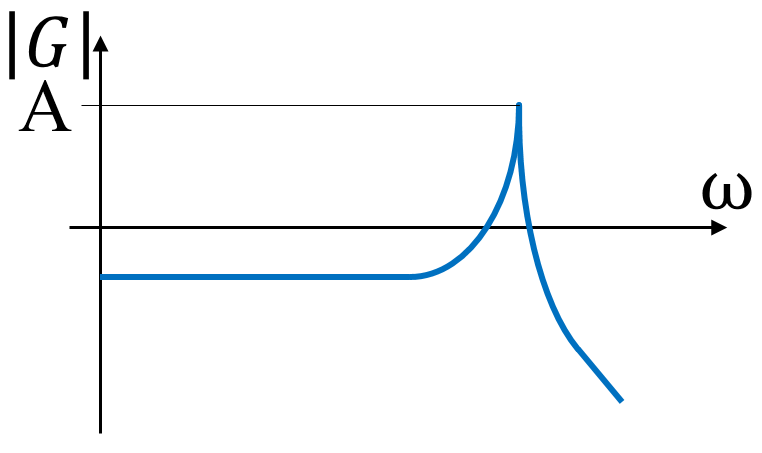
\includegraphics[width=0.25\textwidth]{./bilder/HInf2.PNG}
	}
	\subfloat[Additive Modellunsicherheit \label{subfig:hinf2}]{
		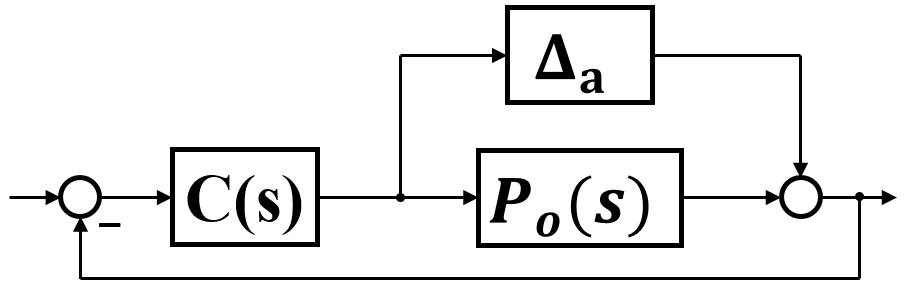
\includegraphics[width=0.25\textwidth]{./bilder/HInf1.PNG}
	}
	\subfloat[Multiplikative Modellunsicherheit \label{subfig:hinf3}]{
		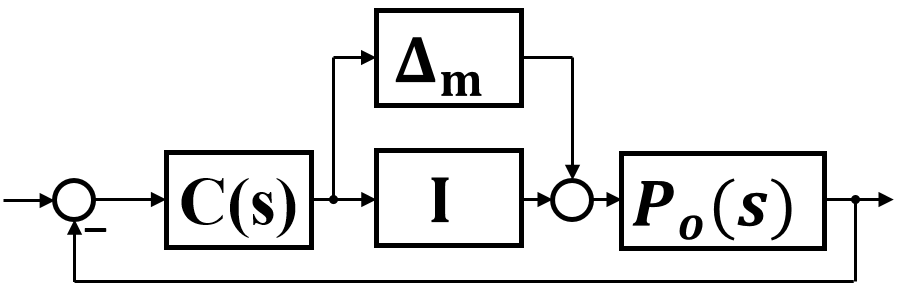
\includegraphics[width=0.25\textwidth]{./bilder/HInf3.PNG}
	}\\
	\label{fig:hinf2}
\end{figure}

\subsection{Staibiltätsanalyse $\rightarrow$ Small-Gain-Theorem}
\subsubsection{Additive Modellunsicherheit}
\begin{itemize}
	\item Modell kann umgezeichnet werden wie in unterstehender Abbildung \ref{subfig:hinf4} gezeigt
	\item In Gleichung \ref{eq:defAddUnsicherheit} ist die Formel für die additive Unsicherheit gezeigt
	\item In Gleichung \ref{eq:addStabilitaet} ist das Kriterium für die Stabilität bei additiver Modellunsicherheit gezeigt
	\item Additive Unsicherheiten können im Nyquist-Diagramm visualisiert werden (siehe Abbildung 9, Skript s.16)
\end{itemize}
\begin{align}
	\label{eq:defAddUnsicherheit}
	\Delta_a(s) &= P(s)-P_0(s)\\
	\label{eq:addStabilitaet}
	\lVert\Delta_a\rVert_\infty &< \frac{1}{\left\lVert\frac{C}{1+P_0C}\right\rVert_\infty} \qquad \Delta_a(s) = P(s)-P_0(s)
\end{align}

\subsubsection{Multiplikative Modellunsicherheit}
\begin{itemize}
	\item Modell kann umgezeichnet werden wie in unterstehender Abbildung \ref{subfig:hinf6} gezeigt
	\item In Gleichung \ref{eq:defMulUnsicherheit} ist die Formel für die Multiplikative Unsicherheit gezeigt
	\item In Gleichung \ref{eq:mulStabilitaet} ist das Kriterium für die Stabilität bei multiplikativer Modellunsicherheit gezeigt
	\item Multiplikative Unsicherheiten können gut in einem Bode-Diagramm dargestellt werden (siehe Abbildung 9, Skript s.16)
\end{itemize}
\begin{align}
\label{eq:defMulUnsicherheit}
\Delta_m(s) &= \frac{P(s)}{P_0(s)}-1\\
\label{eq:mulStabilitaet}
\lVert\Delta_m\rVert_\infty &< \frac{1}{\left\lVert\frac{P_0C}{1+P_0C}\right\rVert_\infty} \qquad 
\end{align}

\begin{figure}[!h]
	\centering
	\subfloat[Modell der additiven Unsicherheit \label{subfig:hinf4}]{
		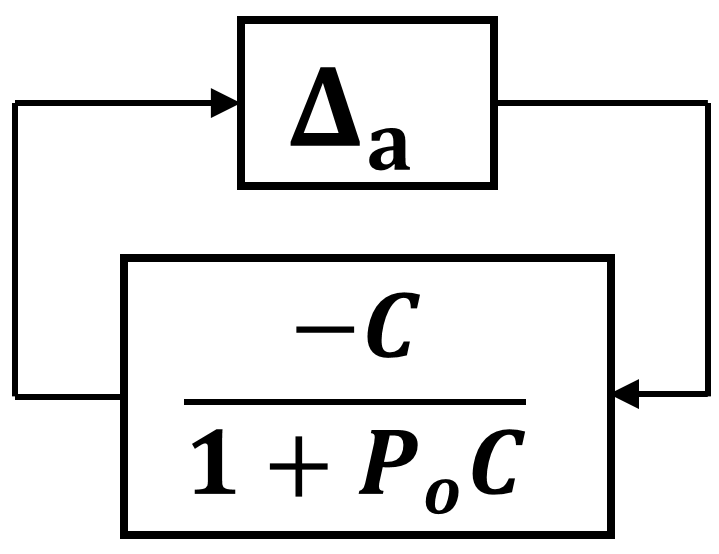
\includegraphics[width=0.15\textwidth]{./bilder/HInf4.PNG}
	}\hspace{0.2\linewidth}
	\subfloat[Modell der multiplikativen Unsicherhei \label{subfig:hinf6}]{
		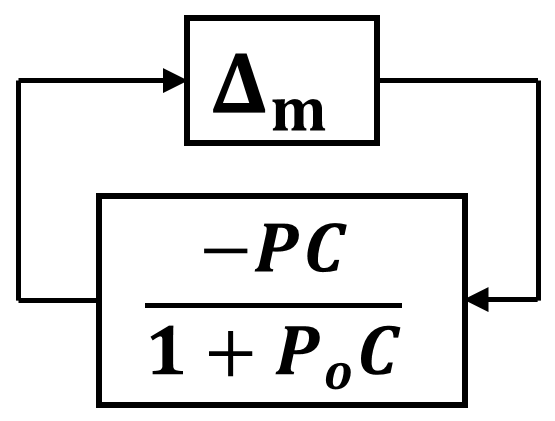
\includegraphics[width=0.15\textwidth]{./bilder/HInf6.PNG}
	}\\
	\caption{ $\text{H}_\infty$-Regelkreise in anderer Darstellung}
	\label{fig:hinf4}
\end{figure}


\subsection{Regelgüte}

\begin{itemize}
	\item Die Funktionen $w_1$, $w_{2a}$ und $w_{2m}$ dürfen nicht mit einem Integrator oder Differentiator beginnen!
	\item Damit dies verhindert wird, werden die Terme $\frac{1}{s}$ resp. $s$ ersetzen durch einen Sehr schnellen Tief-, resp. Hochpass, siehe nachfolgendes Beispiel.
	\item Damit werden Probleme in Berechnung bei $s=0$ verhindert und korrigierte Funktion befriedigt Kriterien für Stabilität
	\item Für die Regelgüte müssen die Gleichungen \ref{eq:GueteAdditiv} und \ref{eq:GueteMultiplikativ} erfüllt sein 
\end{itemize}
\begin{align}
	\label{eq:GueteAdditiv}
	\left\lVert w_{2a}  \frac{C}{1+PC}\right\rVert_\infty < 1\\
	\label{eq:GueteMultiplikativ}
	\left\lVert w_{2m} \frac{PC}{1+PC}\right\rVert_\infty<1
\end{align}

\begin{figure}[!h]
	\centering
	\subfloat[Modell für die Regelgüte mit allen verwendeten Grössen \label{subfig:hinf8}]{
		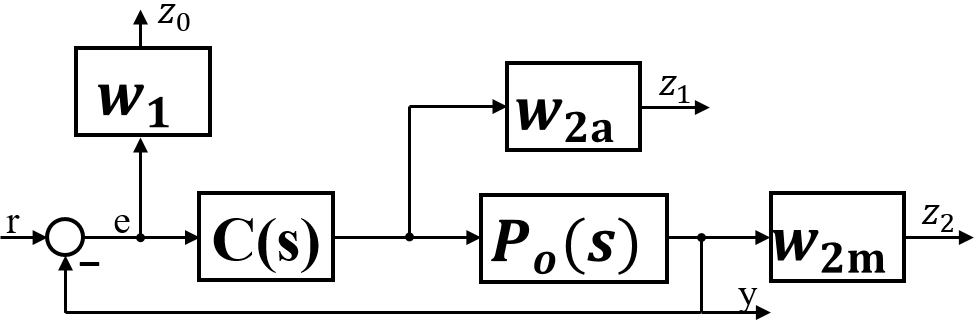
\includegraphics[width=0.35\linewidth]{./bilder/HInf8.PNG}
	}\quad
	\subfloat[Kritische Distanz im Nyquist-Diagramm \label{subfig:hinf7}]{
		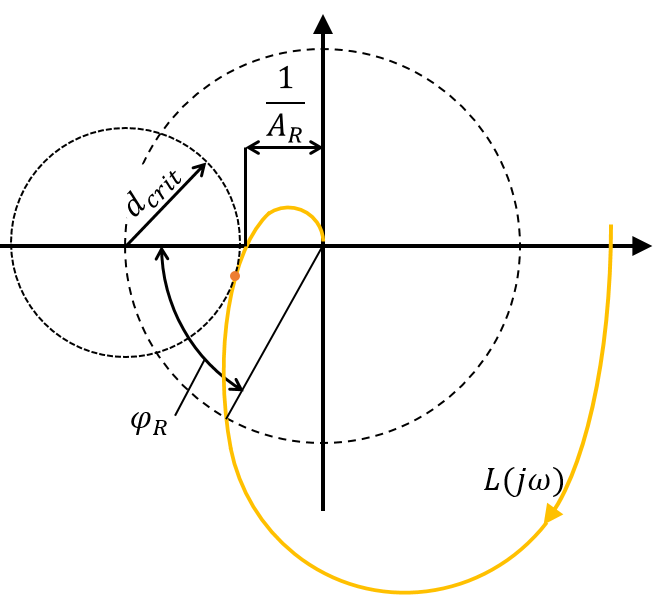
\includegraphics[width=0.27\linewidth]{./bilder/HInf7.PNG}
	}\quad
	\subfloat[Amplitudengang von $S$ und $w_1$  \label{subfig:hinf9}]{
		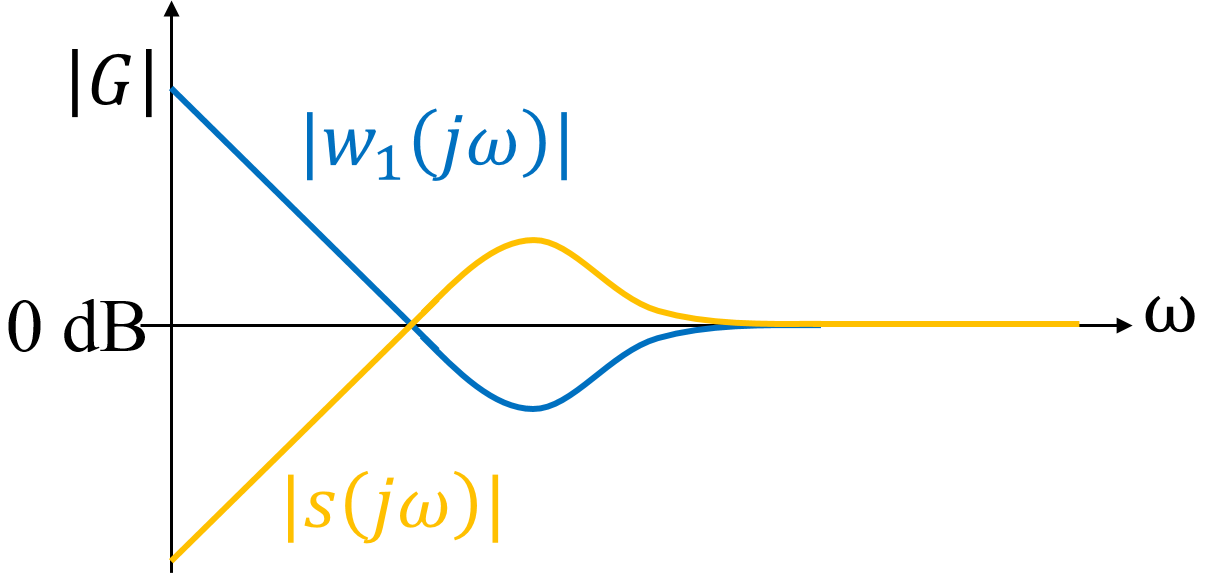
\includegraphics[width=0.27\linewidth]{./bilder/HInf9.PNG}
	}
	\caption{Verschiedene Bilder zu Regelgüte und Senitivitätsfunktion}
	\label{fig:hinf7}
\end{figure}

\begin{tabularx}{\linewidth}{p{0.5\linewidth} p{0.5\linewidth}}
	\textbf{Integrator } bei $\omega=0$	&\textbf{Differentiatior} bei $\omega=0$		\\
	%Zeile 2 mit Allen Bildern
	\includegraphics[width=.5\linewidth]{bilder/hinf12}&
	\includegraphics[width=.5\linewidth]{bilder/hinf11}\\
	%Zeile 2
	%Zeile 3 Mit den Formeln
	\begin{equation*}
	w_1(s) =\frac{1}{s} \quad\Rightarrow w_1(s) = \frac{1}{s+10^{-5}}
	\end{equation*}&
	\begin{align*}
	w_{2a}=\frac{7.5s}{(s+1)(s+15)}\quad\Rightarrow w_{2a} = \frac{0.0075s(s+1000)}{(s+1)(s+15)}
	\end{align*}
\end{tabularx}


\subsubsection{Sensitivitätsfunktion}
\begin{itemize}
	\item $S=$ Sensitivität entspricht dem Übergang von $r$ auf $e$ oder von $d$ auf $y$
	\item Die kritische Distanz maximieren geht einher mit dem Minimieren der $\lVert\text{S}\rVert_\infty$
	\item Erinnerung: $L(s) = P(s)\cdot C(s)$ und wird im open-Loop eingetragen
	\item Robuste Regler zielen darauf ab die kritische Distanz zu maximieren (also $\lVert S \rVert_\infty$ zu minimieren
%?	\item Wird der Amplitudengang von $S(j\omega)$ an der 0-dB-Linie gespiegelt gibt sich gerade der Amplitudengang von $w_1(j\omega)$
	\item Die Funktion $w_1$ ist eine Gewichtungsfunktion (siehe Abbildung \ref{subfig:hinf8}).
	\begin{itemize}
		\item Bei einer Resonanz von $S$ bei $w_1$ eine Zusätzliche Polstelle bei der ca. doppelten Resonanzfrequenz einführen
	\end{itemize}
	\item Die Bode Integralrelation besagt, dass für die Sensitivitätsfunktion die Fläche unterhalb der 0 dB-Linie gleich sein muss wie die Fläche oberhalb der 0 dB-Linie. 
	\begin{itemize}
		\item [\textbf{Achtung:}] Das Flächenverhältnis muss identisch sein, wenn $\omega$ nicht logarithmisch dargestellt wird!
		\item Gezeigt in Abbildung \ref{fig:hinf10}
		\item Je höher (und dadurch kürzer) die orange Fläche ist, desto schneller wird der Regler. Diese Geschwindigkeit geht auf kosten der Stabilität.
	\end{itemize}
\end{itemize}
\begin{align*}
	d_\text{crit}&= \frac{1}{\lVert S \rVert_\infty} \qquad \text{ und } \qquad S(j\omega)=\frac{1}{1+L(J\omega)} = \frac{1}{1+P(j\omega)\cdot C(j\omega)}\\
	T(s) &= \frac{L(s)}{1+L(s)}
\end{align*}
\begin{figure}[!h]
	\centering
	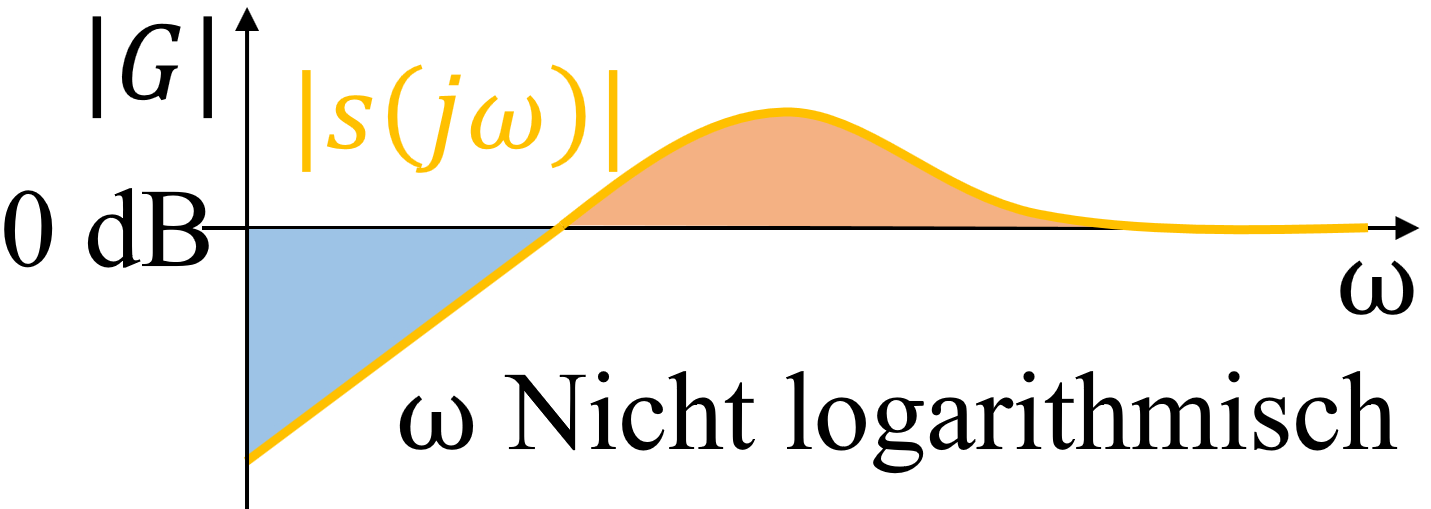
\includegraphics[width=0.2\linewidth]{bilder/HInf10}
	\caption{Trade-Off zwischen Stabilität und Geschwindigkeit}
	\label{fig:hinf10}
\end{figure}

\subsubsection{Gemischter Senitivitätsanspruch}
\begin{itemize}
	\item Funktion soll sowohl Sensitivität des Fehlers, wie auch die additive, oder multiplikative Unsicherheit berücksichtigen
	\item Die Matrix entspricht der Übertragung von $r$ nach $z$
	\item Für Additive Modellunsicherheit Formel \ref{eq:mixedApproachAdd}
	\item Für Multiplikative Modellunsicherheit Formel \ref{eq:mixedApproachMul}
\end{itemize}
\begin{align}
	\label{eq:mixedApproachAdd}
	\left\lVert\begin{bmatrix}
		w_1\frac{1}{1+PC}\\
		w_{2a}\frac{C}{1+PC}
	\end{bmatrix}\right\rVert_\infty <1 \qquad \text{Übertragungsfunktion von }r\text{ nach } \begin{bmatrix}
		z_0\\z_1
	\end{bmatrix}\\
		\label{eq:mixedApproachMul}
	\left\lVert\begin{bmatrix}
	w_1\frac{1}{1+PC}\\
	w_{2m}\frac{PC}{1+PC}
	\end{bmatrix}\right\rVert_\infty <1 \qquad \text{Übertragungsfunktion von }r\text{ nach } \begin{bmatrix}
	z_0\\z_2
	\end{bmatrix}
\end{align}

\subsection{Linear Fractional Transformation (LFT)}
\begin{itemize}
	\item Die LFT von $P$ und $\Delta$ wird geschrieben als $\mathcal{F}\left(P,\Delta\right)$
	\item Für ein SISO-System ist es eine bilineare Transofrmation
	\item Eingänge von Ausserhalb nur in $P$ einführen, falls nötig hindruch passieren mit einer Einheitsmatrix
	\item Entgegen der Abbildung können auch mehrere Eingänge hinein kommen
	\item Beim Umschreiben eines Systems zum LFT alle $P_i$ und alle $C_i$ zusammenfassen
	\item Vorgehen zum erstellen der Matrix $P$
	\begin{itemize}
		\item Achtung: Dieses Vorgehen ist nur sinngemäss beschrieben, aus Zeitgründen und fehlendem Verständnis, wird diese Zusammenfassung hier gewisse Fehler aufweisen. 
		\item [1.] In System in klassischer Schreibweise: Boxen um die zusammenzufassenden Blöcke zeichnen (Systemgrenzen bestimmen)
		\item [2.] Ein- und Ausgänge definieren 
		\item [3.] Alles was in das System von Aussen kommt muss über Block $P$ eingespiesen werden
		\item [4.] $\dot{x} = Px$ wobei $\dot{x}$ dem nächsten Schritt entspricht (analog dem Aufbau der Matrix $A$ )
	\end{itemize}
	\item Beispiel siehe Beispiel unten (entsprechend der Aufgabe 1 von \glqq Robust Control \grqq)
\end{itemize}


\begin{figure}[h!]
	\centering
	\begin{minipage}{0.25\linewidth}
		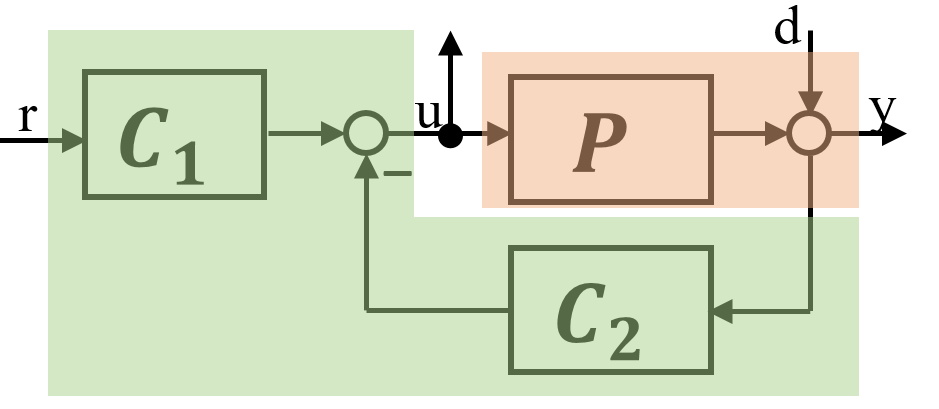
\includegraphics[width=1\linewidth]{bilder/LFT3}
	\end{minipage}
	\begin{minipage}{0.25\linewidth}
		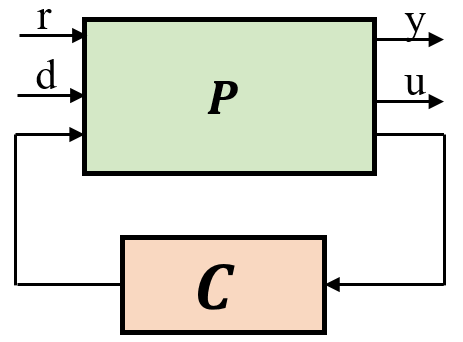
\includegraphics[width=.75\linewidth]{bilder/LFT4}
	\end{minipage}
	\begin{minipage}{0.45\linewidth}
		\footnotesize
			\begin{equation*}
		C: u = \begin{bmatrix}
		C_1 & -C_2
		\end{bmatrix} \begin{bmatrix}
		r\\y
		\end{bmatrix}				
		\end{equation*}
		\begin{equation*}
		\begin{bmatrix}
		y\\u\\y\\r
		\end{bmatrix} = \begin{bmatrix}
		0 & I & P\\
		0 & 0 & I\\
		I & 0 & 0\\
		0 & I & P
		\end{bmatrix}\begin{bmatrix}
		r\\d\\u
		\end{bmatrix}
		\end{equation*}
	\end{minipage}
\end{figure}

\begin{figure}[!h]
	\begin{minipage}{0.25\linewidth}
		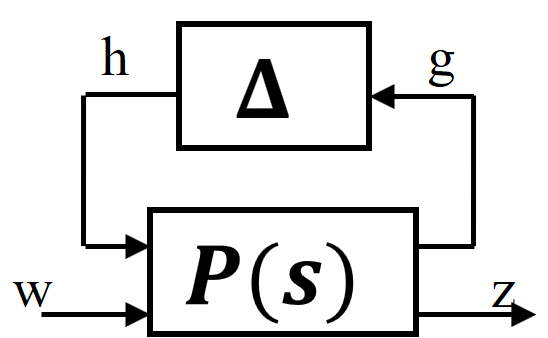
\includegraphics[width=.75\linewidth]{bilder/LFT1}
	\end{minipage}
	\begin{minipage}{0.35\linewidth}
		\footnotesize
		\textbf{Additive Modellunsicherheit}
		\begin{equation*}
			P = \begin{bmatrix}
				0 	& I\\
				I	& P_0
			\end{bmatrix}
		\end{equation*}
	\end{minipage}
	\begin{minipage}{0.35\linewidth}
		\footnotesize
		\textbf{Multiplikative Modellunsicherheit}
		\begin{equation*}
			P = \begin{bmatrix}
				0 	& P_0\\
				I	& P_0
			\end{bmatrix}
		\end{equation*}
	\end{minipage}
\end{figure}
\newpage
\section{Nicht Lineare Systeme}
\subsection{Basics}
\begin{itemize}
	\item Superpositionsprinzip gilt nicht
	\item Stabilität ist lokale Eigenschaft
	\item Finite Escape time (Wert in endlicher Zeit bei $\infty$)
	\item Viele Beharrungszustände
	\item Chaotische Systeme existieren
\end{itemize}
\subsection{Bestimmung der Stabilität}
\subsubsection{Layapunov 1. Methode}
\begin{itemize}
	\item System um Beharrungszustand linearisieren
	\begin{itemize}
		\item Stabilität im linearisierten System $\Rightarrow$ Stabilität um Beharrungszustand
	\end{itemize} 
	\item Sind die Realanteile der Eigenwerte  $< 0$ ist das System an dem Punkt stabil um den Beharrungszustand
	\item Sind die Realanteile der Eigenwerte  $> 0$ ist das System an dem Punkt instabil um den Beharrungszustand
	\item Siehe für Beispiel Gleichung \ref{eq:Layapunov1} (ist Aufgabe 1 aus \glqq Nicht lineare Systeme I\grqq)
	\item Linearisieren an einem Punkt, entspricht der Jacobi-Matrix mit den Werten dieses Punktes Eingesetzt $\rightarrow$ Matrix $A$
\end{itemize}
\begin{align}
	\label{eq:Layapunov1}
	\dot{\underline{x}} &= f(\underline{x})
	\begin{bmatrix}
		x_1\\
		x_2
	\end{bmatrix} = \begin{bmatrix}
		x_2\\
		-\frac{r}{m}x_2-\frac{g}{l}x\sin(x_1)
	\end{bmatrix}\\
	J &= \left.\begin{bmatrix}
		\frac{\partial f_1(x1,x2)}{\partial x1}	& \frac{\partial f_1(x1,x2)}{\partial x2}\\
		\frac{\partial f_2(x1,x2)}{\partial x1} &\frac{\partial f_2(x1,x2)}{\partial x2}
	\end{bmatrix}\right\lvert_{\begin{matrix}
		x_1\\x_2
	\end{matrix}}
\end{align}

\subsubsection{Layapunov 2. Methode}
\begin{itemize}
	\item Laypunov-Funktion $V(x)$, damit diese zulässig ist, müssen folgende Bedingungen erfüllt sein:
	\begin{itemize}
		\item []$V\left(\underline{0}\right) = 0$
		\item []$V\left(\underline{x}\right) > 0$
	\end{itemize}	
	\item Reminder: $\underline{x}$ sind Funktionen $\rightarrow$ Ableitung von $V(x)$ mit Kettenregel
	\begin{itemize}
		\item [z.B.] $V(\underline{x}) = x_1^2+x_2^2 \qquad\Rightarrow \dot{V}(x) = 2x_1\dot{x}_1 + 2x_2\dot{x}_2$
	\end{itemize}
	\item Ein System ist um einen Bereich (um $\underline{x}$)lokal stabil, wenn $\dot{V}\left(\underline{x}\right) < 0$ erfüllt ist 
\end{itemize}

\subsubsection{Layapunov in Linearen Systemen}
\begin{itemize}
	\item In Linearen System können folgende Abgewandelte Bedienungen angewendet werden, wenn folgendes erfüllt ist:
	\begin{itemize}
		\item $P>0 \rightarrow$ Positiv definite Matrix (alle Eigenwerte von $P>0$)
	\end{itemize}
	\item Gleichtung \ref{eq:Layapunov2} ist die Layapunov-Gleichung
\end{itemize}
\begin{align}
	V(x) &=x^TPx\\
	\dot{V}(x) &= x^TA^TPx+x^TPAx < 0\\
	\label{eq:Layapunov2}
	A^T+PA&=-Q\\
	Q&=B^TB	\qquad \text{Mass für Beobachtbarkeit}\\
	Q&=CC^T	\qquad	\text{Mass für Steuerbarkeit}
\end{align}

\subsection{Popov-Kreiskriterium}
\begin{itemize}
	\item Miteinkalkulieren einer Gewissen Nichtlinearität der Regelstrecke
	\begin{itemize}
		\item Begrenzt durch zwei Lineare Funktionen
	\end{itemize}
	\item Nichtlinearität darf keine Sprünge enthalten
	\item Nichtlinearität innerhalb eines Bereiches Eingrenzen
	\begin{itemize}
		\item Dieser Bereich wird mit zwei Steigungen beschrieben, $a$ und $b$
	\end{itemize}
	\item Das Popovkriterium ist eine Erweiterung des Nyquist-Kriterium
	\begin{itemize}
		\item In diesem Fall ist es ein Kreis, definiert durch die Steigungen der begrenzenden Funktionen
		\item Siehe für den Zusammenhang  Abbildung \ref{fig:Popov1} und \ref{fig:Popov3}
		\item Pro instabilem Pol muss die Frequenzlinie den Kreis einmal im Gegenuhrzeigersinn umkreisen, ohne die Fläche zu berühren.
	\end{itemize}
	\item Die Wichtigsten Sonderfälle sind in Abbildung \ref{fig:PopovSonderfaelle} gezeigt. 
\end{itemize}
\begin{figure}[!h]
	\footnotesize
	\begin{minipage}{0.25\linewidth}
		\footnotesize
		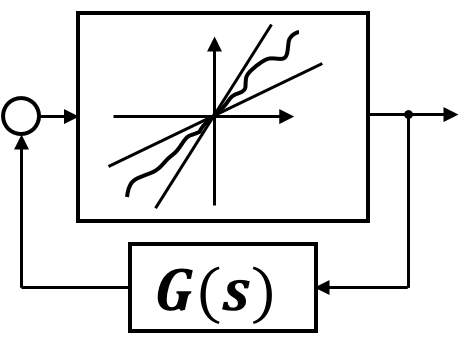
\includegraphics[width=1\linewidth]{./bilder/Popov2.png}
		\caption{Ersatzschaltbild von Popov}
	\end{minipage}\hspace{0.1\linewidth}
	\begin{minipage}{0.25\linewidth}
		\footnotesize
		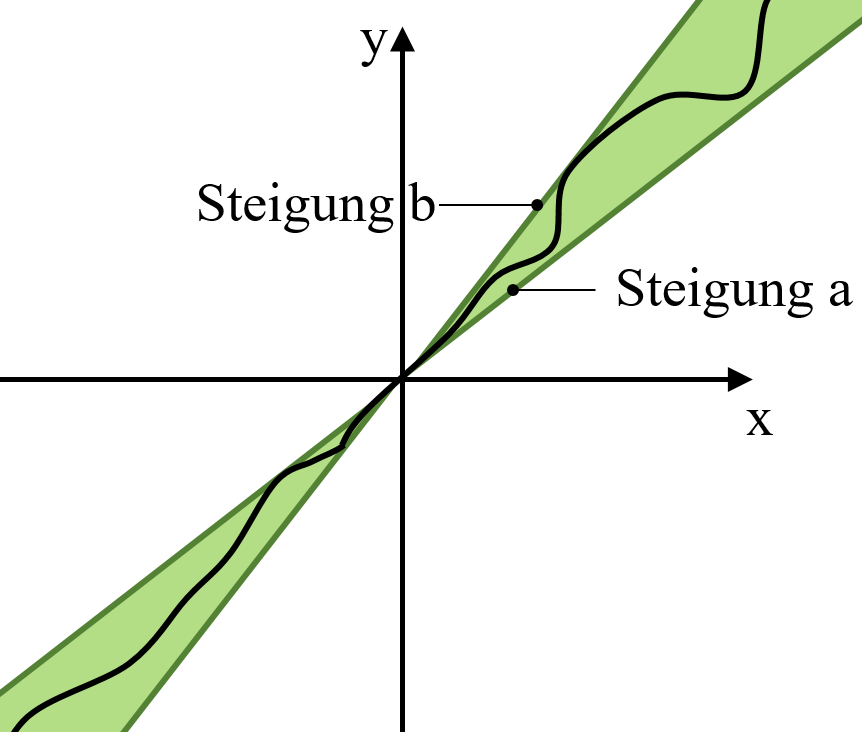
\includegraphics[width=1\linewidth]{./bilder/Popov1.png}
		\label{fig:Popov1}
		\caption{Begrenzende Funktionen umgeben die Nichtlinearität}
	\end{minipage}\hspace{0.1\linewidth}
	\begin{minipage}{0.25\linewidth}
		\footnotesize
		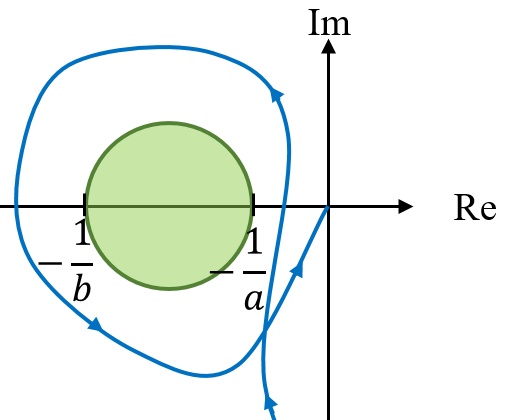
\includegraphics[width=1\linewidth]{./bilder/Popov3.png}
		\label{fig:Popov3}
		\caption{Zusammenhang zwischen begrenzenden Funktionen und Nyquist diagramm}
\end{minipage}
\end{figure}

\begin{figure}[!h]
	\centering
	\begin{minipage}{0.15\linewidth}
		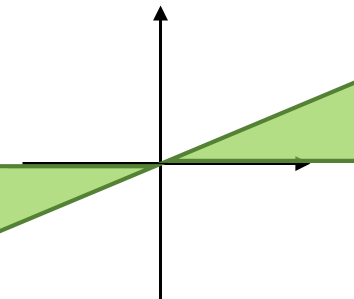
\includegraphics[width=1\linewidth]{./bilder/Popov4.png}.
	\end{minipage}\hspace{0.05\linewidth}$\Rightarrow$\hspace{0.05\linewidth}
	\begin{minipage}{0.15\linewidth}
		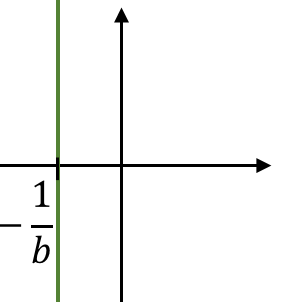
\includegraphics[width=1\linewidth]{./bilder/Popov5.png}.
	\end{minipage}\hspace{.1\linewidth}
	\begin{minipage}{0.15\linewidth}
		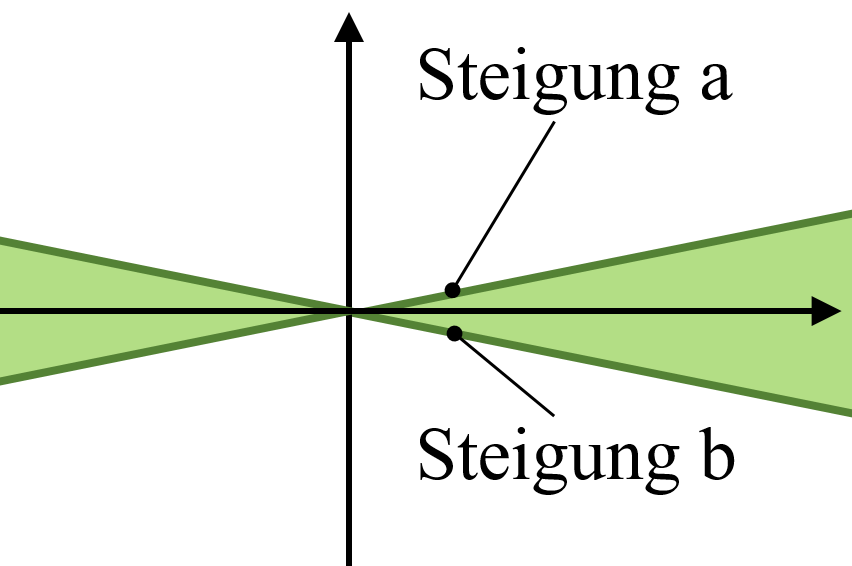
\includegraphics[width=1\linewidth]{./bilder/Popov6.png}.
	\end{minipage}\hspace{0.05\linewidth}$\Rightarrow$\hspace{0.05\linewidth}
	\begin{minipage}{0.15\linewidth}
		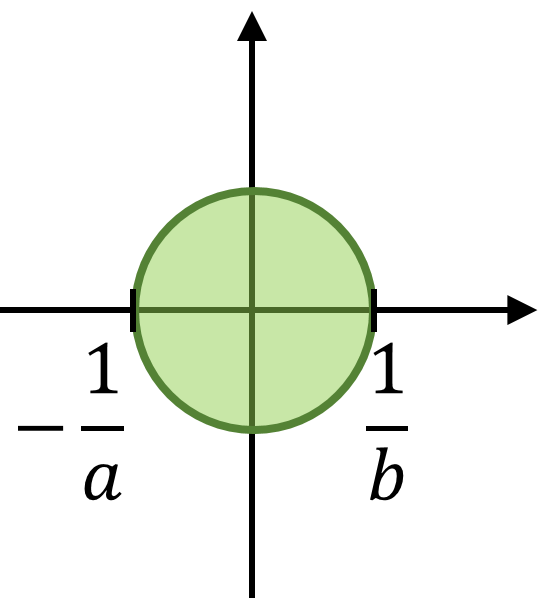
\includegraphics[width=1\linewidth]{./bilder/Popov7.png}.
	\end{minipage}	
	\label{fig:PopovSonderfaelle}
	\caption{Sonderfälle bei der Anwendung des Popov-Stabilitätskriterium}
\end{figure}

\subsection{Beschreibungsfunktionsmethode}
\begin{itemize}
	\item Beschreibungsfunktion wird mit $N(A)$ bezeichnet, siehe Anhang \ref{sec:AnhBeschreibungsf}
	\item Ziel: Die Beschreibungsfunktion beschreibt die Nichtlinearität des Systems
	\begin{itemize}
		\item Siehe Anhang für die wichtigsten Beschreibungsfunktionen
	\end{itemize}
	\item Totband:
	\begin{itemize}
		\item Erst wenn ein gewisser Fehler ($e$) Überschritten ist, passiert dieser das Totbandglied
		\item Der Ausgang nach dem Totband ist jeweils um 1/2 des Fehlers versetzt
		\item Gezeigt in Abbildung \ref{fig:totband}
	\end{itemize}
	\item Relais
	\begin{itemize}
		\item Schaltet jeweils bei 0-Durchgang des Eingangs
		\item Amplitude am Ausgang springt bei Nulldurchgang, auf die jeweilige Seite 
	\end{itemize}
\end{itemize}
\begin{figure}[!h]
	\centering
	\includegraphics[width=0.5\linewidth]{./bilder/totband.png}
	\label{fig:totband}
	\caption{Symbol des Totbandes und dessen Ein- und Ausgangssignal}
\end{figure}

\subsubsection{Grenzzyklus}
\begin{itemize}
	\item Regelkreis mit Maximaler Verstärkung 
	\item Phase ist \ang{-180}
	\item Der Grenzzyklus ist der Schnittpunkt gemäss Abbildung \ref{fig:Beschreibungsf}, gemäss Formel \ref{eq:Beschreibungsf1}
	\item Ein Grenzzyklus existiert, wenn
	\begin{itemize}
		\item die Linie der Beschreibungsfunktion im Nyquist-Diagramm schneidet die Frequenzlinie (des Open-Loops) von rechts nach links
		\item Dabei ist die Betrachtung aus sicht der zunehmenden Frequenz
		\item Siehe Beispiel in Abbildung \ref{fig:Beschreibungsf}
	\end{itemize}
	\item Es ist das $A$ gesucht, dies entspricht der Amplitude des Eingangssignal
	\begin{itemize}
		\item In diesem Fall $N(A)$ bestimmen mit Schnittpunkt und das $A$ ausrechnen
	\end{itemize}
	\item Oder die Grenzfrequenz ist gesucht
	\begin{itemize}
		\item Bestimmen durch Schnittpunkt gemäss Formel \ref{eq:Beschreibungsf1}
	\end{itemize}
	\item Oder die Zulässige Verstärkung des Regelkreises $\lvert G(j\omega)\rvert$ 
	\begin{itemize}
		\item Formel \ref{eq:Beschreibungsf1} auflösen nach $G(j\omega)$
	\end{itemize}
\end{itemize}

\begin{figure}[!h]
	\begin{minipage}{0.6\linewidth}
		\centering
		\includegraphics[width=.4\linewidth]{./bilder/Beschreibungsfunk1.png}
		\caption{Schnittpunkt ist bei der Grenzfrequenz, Beispiel für ein Relais}
		\label{fig:Beschreibungsf}
	\end{minipage}
	\begin{minipage}{0.3\linewidth}
		\begin{align}
		\label{eq:Beschreibungsf1}
		\frac{-1}{N(A)} = G_{Ol}(j\omega)
		\end{align}
	\end{minipage}
\end{figure}

\clearpage
\newpage
\section{Verschiedene Transformationen}
\begin{minipage}{13.5cm}
\subsection{Berechnung}
\tiny
\begin{tabular}{|l|l|l|}
\hline
  \textbf{Transformation}
  & \textbf{Vorwärts}
  & \textbf{Rückwärts} \\
\hline
  Fourier-Reihe
  & $c_k=\frac{1}{T}\int_0^T{f(t) e^{-jk\omega_1 t}dt}$
  & $f(t) = \sum\limits_{k = -\infty}^{\infty} c_k  e^{j k \omega_1 t}$ \\
\hline
  Fourier-Integral
  & $F(\omega) = \int\limits_{-\infty}^{\infty} f(t)e^{-j\omega t}dt$
  & $f(t) =  \frac{1}{2\pi}\int\limits_{-\infty}^{\infty}
    F(\omega)e^{j\omega t}d\omega$ \\
\hline
  Laplace-Transformation
  & $F(s)=\int\limits_0^\infty f(t)e^{-st}dt$
  & Polynomdivision $\Rightarrow$ Partialbruchzerlegung $\Rightarrow$ Tabelle!\\
\hline
  Diskrete Fouriertransformation
  & $F(k) = \sum\limits_{n=0}^{N-1} f(n) e^{-j 2 \pi \frac{n}{N} k}$
  & $f^*(k) = \frac{1}{N} DFT(F^* (k))$\\
\hline
  Z-Transformation ($z = e^{j s T}$)
  & $F(z) = \sum\limits_{n=0}^{\infty} f(n) z^{-n}$
  & Polynomdivision $\Rightarrow$ Partialbruchzerlegung $\Rightarrow$ Tabelle!\\
\hline
\end{tabular}
\normalsize
\end{minipage}
\begin{minipage}{5.5cm}
\subsection{Pol/Nullstellentransfo}
\includegraphics[width=5.5cm]{bilder/ImagAchse-Einheitskreis.png}
\end{minipage}

\section{Eigenschaften von Fourier- und Z-Transformation}
\tiny
\renewcommand{\arraystretch}{1.1}
\begin{tabular}{|p{3.2cm}||p{1.5cm}|p{1.8cm}||p{2.5cm}|p{2.5cm}||p{1.7cm}|p{3cm}|}
\hline
\textbf{Bezeichnung}
  & \multicolumn{2}{|c||}{\textbf{Zeitbereich}}
  & \multicolumn{2}{|c||}{\textbf{Kontinuierlicher Frequenzbereich}}
  & \multicolumn{2}{|c|}{\textbf{Diskreter Frequenzbereich}} \\
  & \textbf{kontinuierlich}
  & \textbf{diskret}
  & \textbf{Fourier-Integral}
  & \textbf{Laplace}
  & \textbf{Diskrete FT}
  & \textbf{Z-Transformation} \\
\hline
\hline
  Linearität
  & $\alpha\cdot f(t) + \beta\cdot g(t)$
  & $\alpha\cdot f(n) + \beta\cdot g(n)$
  & $\alpha\cdot F(\omega) + \beta\cdot G(\omega)$
  & $\alpha\cdot F(s) + \beta\cdot G(s)$
  & $\alpha\cdot F(n) + \beta\cdot G(n)$
  & $\alpha\cdot F(z) + \beta\cdot G(z)$\\
\hline
  "Ahnlichkeit / Zeitskalierung bzw. Spiegelung an Y-Achse
  &	$f(\alpha t)$
  & $f(-n)$
  & $\frac{1}{|\alpha|}F \left (\frac{\omega}{\alpha} \right)$
  & $\frac{1}{\alpha}F \left (\frac{s}{\alpha} \right )$
  & $F(-n)$
  & $F(z^{-1})$\\
\hline
  Dämpfung
  & -
  & $e^{dn} f(n)$
  & -
  & -
  & -
  & $F(z e^{d})$ \\
\hline
  Verschiebung im Zeitbereich
  & $f(t\pm t_0)$
  & $f(n \pm n_0)$
  & $e^{\pm j\omega t_0} F(\omega)$
  & $F(s)e^{\pm t_0 s}$
  & $e^{\pm j\frac{n}{N}2 \pi n_0} F(n)$
  & $z^{\pm n_0} F(z)$\\
\hline
  Verschiebung im Frequenzbereich
  & $f(t)e^{\mp\alpha t}$
  & $f(n) e^{\mp j \frac{n}{N} 2 \pi n_0}$
  & $F(\omega\pm \alpha)$
  & $F(s\pm\alpha)$
  & $F(n \pm n_0)$
  & $F(z \pm n_0)$\\
\hline
  Faltung im Zeitbereich
  &	$f(t) \ast g(t)$
  & $f(n) \ast g(n)$
  & $F(\omega) \cdot G(\omega)$
  & $F(s) \cdot G(s)$
  & $F(n) \cdot G(n)$
  & $F(z) \cdot G(z)$ \\
\hline
  Faltung im Frequenzbereich
  &	$f(t) \cdot g(t)$
  & $f(n) \cdot g(n)$
  & $\frac{1}{2\pi} F(\omega) \ast G(\omega)$
  & $\frac{1}{2\pi} F(s) \ast G(s)$
  & $\frac{1}{N} F(n) \ast G(n)$
  & $\frac{1}{N} F(z) \ast G(z)$\\
\hline
  Ableitungen im Zeitbereich bzw. Differenzenbildung
  & $\frac{\partial^n f(t)}{\partial t^n}$
  & $\Delta^k f(n)$
  & $(j\omega)^n F(\omega)$
  & $s^nF(s)-s^{n-1}f(0+)-s^{n-2}\frac{\partial f(0+)}{\partial t}-\ldots
 			-s^0\frac{\partial^{n-1} f(0+)}{\partial t^{n-1}}$
  &
  & $(1-z^{-1})^k F(z)$ \\
\hline
  Ableitung im Frequenzbereich
  & $(-t)^k\cdot f(t)$
  & $n f(n)$
  & $j^k \frac{-\partial^k F(\omega)}{\partial \omega^k}$
  & $\frac{\partial^k F(s)}{\partial s^k}$
  &
  & $-z \frac{\partial F(z)}{\partial z}$ \\
\hline
  Integration bzw. Summierung
  & $\int\limits_{-\infty}^t f(\tau)d\tau$
  & $\sum\limits_{n=0}^{k} f(n)$
  & $\frac{F(\omega)}{j\omega}+F(0)\pi\delta(\omega)$
  & $\frac{F(s)}{s}$
  &
  & $\frac{1}{1-z^{-1}} F(z)$ \\
\hline
  Anfangswert
  & $\lim\limits_{t\rightarrow 0} f(t)$
  & $f(0)$
  &
  & $\lim\limits_{s\rightarrow \infty} sF(s)$
  &
  & $\lim\limits_{z \rightarrow \infty} F(z)$ \\
\hline
  Endwert
  &	$\lim\limits_{t\rightarrow \infty} f(t)$
  & $\lim\limits_{n\rightarrow \infty} f(n)$
  &
  & $\lim\limits_{s\rightarrow 0} sF(s)$
  &
  & $\lim\limits_{z \rightarrow 1} (1-z^{-1} F(z))$\\
\hline
  Stabilität
  & -
  & -
  & -
  & Pole in LHE
  &
  & Pole innerhalb Einheitskreis \\
\hline
  Kausalität
  & -
  & -
  & A- \& Kausal
  & Nur Kausal
  &
  & $\lim\limits_{z \rightarrow \infty} z^{-1} F(z) = 0$ \\
\hline
\hline
  Spezial
  & \multicolumn{3}{l||}{
      Bessel-Theorem \qquad
      $\int\limits_{-\infty}^{\infty}f(t)g^{\ast}(t)dt =
         \frac{1}{2\pi}
         \int\limits_{-\infty}^{\infty}F(\omega)G^{\ast}(\omega)d\omega$}
  & \multicolumn{3}{|l|}{
      Parseval-Theorem \qquad
      $W = \int\limits_{-\infty}^{\infty}|f(t)|^2 dt = \frac{1}{2\pi}
      \int\limits_{-\infty}^{\infty}|F(\omega)|^2 d\omega$
    }\\
\hline
\end{tabular}
\renewcommand{\arraystretch}{1}\\
\normalsize

\begin{minipage}{11cm}
	\includegraphics[height=11cm]{bilder/Z-Lexikon.png}
\end{minipage}
\begin{minipage}{8cm}
	\includegraphics[width=8cm]{bilder/IIR-ArbeitsschritteundVarianten.png}
\end{minipage}
\newpage
\section{Matrizenrechnung}
\scriptsize


\subsection{Determinante}

	\textbf{3x3 Matrix}
	$$ \det \begin{bmatrix} a_{11} & a_{12} & a_{13} \\ a_{21} & a_{22}& a_{23} \\
	a_{31} & a_{32} & a_{33} \end{bmatrix} \\ = a_{11} a_{22} a_{33} + a_{12}
	a_{23} a_{31} + a_{13} a_{21} a_{32} - a_{13} a_{22} a_{31} - a_{12} a_{21}
	a_{33} - a_{11} a_{23} a_{32}.  $$
	
	\textbf{Dreiecksmatrix} - Alle Elemente entweder ober- oder unterhalt der Hauptdiagonale $= 0$
	$$\det A =a_{11}\cdot a_{22}\dotsb a_{nn} \quad  \quad \text{Die Det. ist das Produkt
	der Hauptdiagonal-Einträge. Gilt somit auch für Diagonalmatritzen.} $$
	
	\textbf{Null $(|A| = 0)$} - Wenn $A$ eine (n,n)-Matrix ist, so wird $|A| = 0$ unter einer der
	folgenden Bedingungen:
	\begin{itemize}
    	\item Zwei Zeilen/Spalten sind linear abhängig (gleich oder ein Vielfaches der anderen).
    	\item Alle Elemente einer Zeile/Spalte sind Null. \\
  	\end{itemize} 
	
	\textbf{Allgemein:}
	$$A\epsilon M_n: \det A =    
	\begin{vmatrix}
    	a_{11} & a_{12}& \ldots & a_{1n}\\
    	a_{21}& &\ldots & \\
    	\ldots \\
    	a_{n1} & & \ldots & a_{nn}    			
    \end{vmatrix}=
	(-1)^{1+1}a_{11}D_{11} + (-1)^{1+2}a_{12}D_{12}+ \ldots +
	(-1)^{1+n}a_{1n}D_{1n}$$
	
	\subsubsection{Unterdeterminante}
	$$D_{11}=
	\begin{vmatrix}
    	a_{22} & \ldots & a_{2n}\\
    	\ldots\\
    	a_{n2}& \ldots & a_{nn}
    \end{vmatrix} 	\\
	D_{12}=
	\begin{vmatrix}
    	a_{21} & a_{23}& \ldots & a_{2n}\\
    	\ldots\\
    	a_{n1}& a_{n3}&\ldots & a_{nn}
    \end{vmatrix}$$\\
	$D_{ij}$ die (n-1)$ \times $(n-1)-Untermatrix von D ist, die durch Streichen der
	i-ten Zeile und j-ten Spalte entsteht.\\
	Diese Methode ist zu empfehlen, wenn die Matrix in einer Zeile oder Spalte
	bis auf eine Stelle nur Nullen aufweisst.
	Dies lässt sich meist mit dem Gausverfahren bewerkstelligen.
	
\subsection{Gaussverfahren}
	Durch Addition und Subtraktion einzelner Zeilen (auch von Vielfachen einer
	Zeile) werden einzelne Stellen auf Null gebracht. zB:\\
	$\begin{bmatrix}
    	a_{11} & a_{12}& \ldots & a_{1n}\\
    	a_{21}& &\ldots & \\
    	\ldots \\
    	a_{n1} & & \ldots & a_{nn}    			
    \end{bmatrix}=
	\begin{bmatrix}
    	a_{11} & a_{12}& \ldots & a_{1n}\\
    	k a_{21}-n a_{11}& ka_{22}-n a_{12}&\ldots & k a_{2n} - n a_{1n}\\
    	\ldots \\
    	a_{n1} & & \ldots & a_{nn}    			
    \end{bmatrix}$ \\
	Die n * erste Zeile wurde von der k * zweiten Zeile abgezogen ($a_{2.}= 
	k a_{2.}- n a_{1.}$)
	
\subsection{Inverse Matrix \small{(Existiert nur wenn Matrix regulär: $\det A \neq 0$)}}
\begin{minipage}{7cm}
	\textbf{2x2 Matrix:}    
	$$ A^{-1} = \begin{bmatrix} a & b \\ c & d \\ \end{bmatrix}^{-1} = \frac{1}{ad
	- bc} \begin{bmatrix} d & -b \\ -c & a \\ \end{bmatrix} $$
\end{minipage}
\begin{minipage}{11cm}
	\textbf{3x3 Matrix:}
  $$  A^{-1} = \begin{bmatrix} a & b & c\\ d & e & f \\ g & h & i \\ \end{bmatrix}^{-1} =
  \frac{1}{\det(A)} \begin{bmatrix} ei - fh & ch - bi & bf - ce \\ fg - di & ai
  - cg & cd - af \\ dh - eg & bg - ah & ae - bd \end{bmatrix} $$
\end{minipage}\\

\textbf{Diagonalmatrix} (Alle Elemente ausserhalb der Hauptdiagonale $= 0$, Elemente auf
Hauptdiagonale sind Eigenwerte $\lambda_i$): \\ 
Alle Elemete elementweise invertieren - Kehrwert. $\quad \Rightarrow \quad $\textit{Gilt nur wenn
alle Elemente auf der Hauptdiagonale $\neq 0$ sind.}\\

\textbf{Allgemein:}\\
	$A^{-1}= \begin{bmatrix}
    	a_{11} & a_{12}& \ldots & a_{1n}\\
    	a_{21}& &\ldots & \\
    	\ldots \\
    	a_{n1} & & \ldots & a_{nn}    			
    \end{bmatrix}^{-1}$
	\begin{enumerate}
		\item $A^T$ bestimmen (Zeilen und Spalten vertauschen) $A^{T}= \begin{bmatrix}
    	a_{11} & a_{21}& \ldots & a_{n1}\\
    	a_{12}& &\ldots & \\
    	\ldots \\
    	a_{1n} & & \ldots & a_{nn}    			
    \end{bmatrix}$	
		\item Bei $A^T$ jedes Element $a_{ij}$ durch Unterdet. $D_{ij}$ mit
		richtigem Vorzeichen ersetzen $A^*=	\begin{bmatrix}
			(-1)^{1+1}D_{11} &  \ldots	& (-1)^{1+n} D_{1n}\\
			\ldots\\
			(-1)^{n+1} D_{n1}& \ldots  & (-1)^{n+n} D_{nn}
		\end{bmatrix}$
		\item $A^{-1} = \frac{A^*}{\det A}$ 
    \end{enumerate}
 
 \subsection{Diagonalisierung}
 	\begin{enumerate}
       \item Eigenwerte $\lambda$ auschrechnen: $\det (A - I_n \lambda)=0$
       \item Eigenvektoren $\vec{v}$ bilden: $(A- \lambda I_n)\vec{v}=0$
       \item Transformationsmatrix: $T= [\vec{v_1} \ldots \vec{v_n}]$
       \item $T^{-1}$ berechnen (Achtung ist A symmetrisch, dh. $A^T=A$ und
       oder alle EV senktrecht zueinander, dann $T^{-1}=T^T$)
       \item $D=\begin{bmatrix}
                	\lambda_1 &0 &0\\
                	0& \lambda_2 &0\\
                	0& 0& \lambda_3
                \end{bmatrix}$
		\item $A^n = T D^n T^{-1}$

     \end{enumerate}
\newpage
\section{Anhang: Beschreibungsfunktionen}
\label{sec:AnhBeschreibungsf}
\begin{minipage}{\linewidth}
	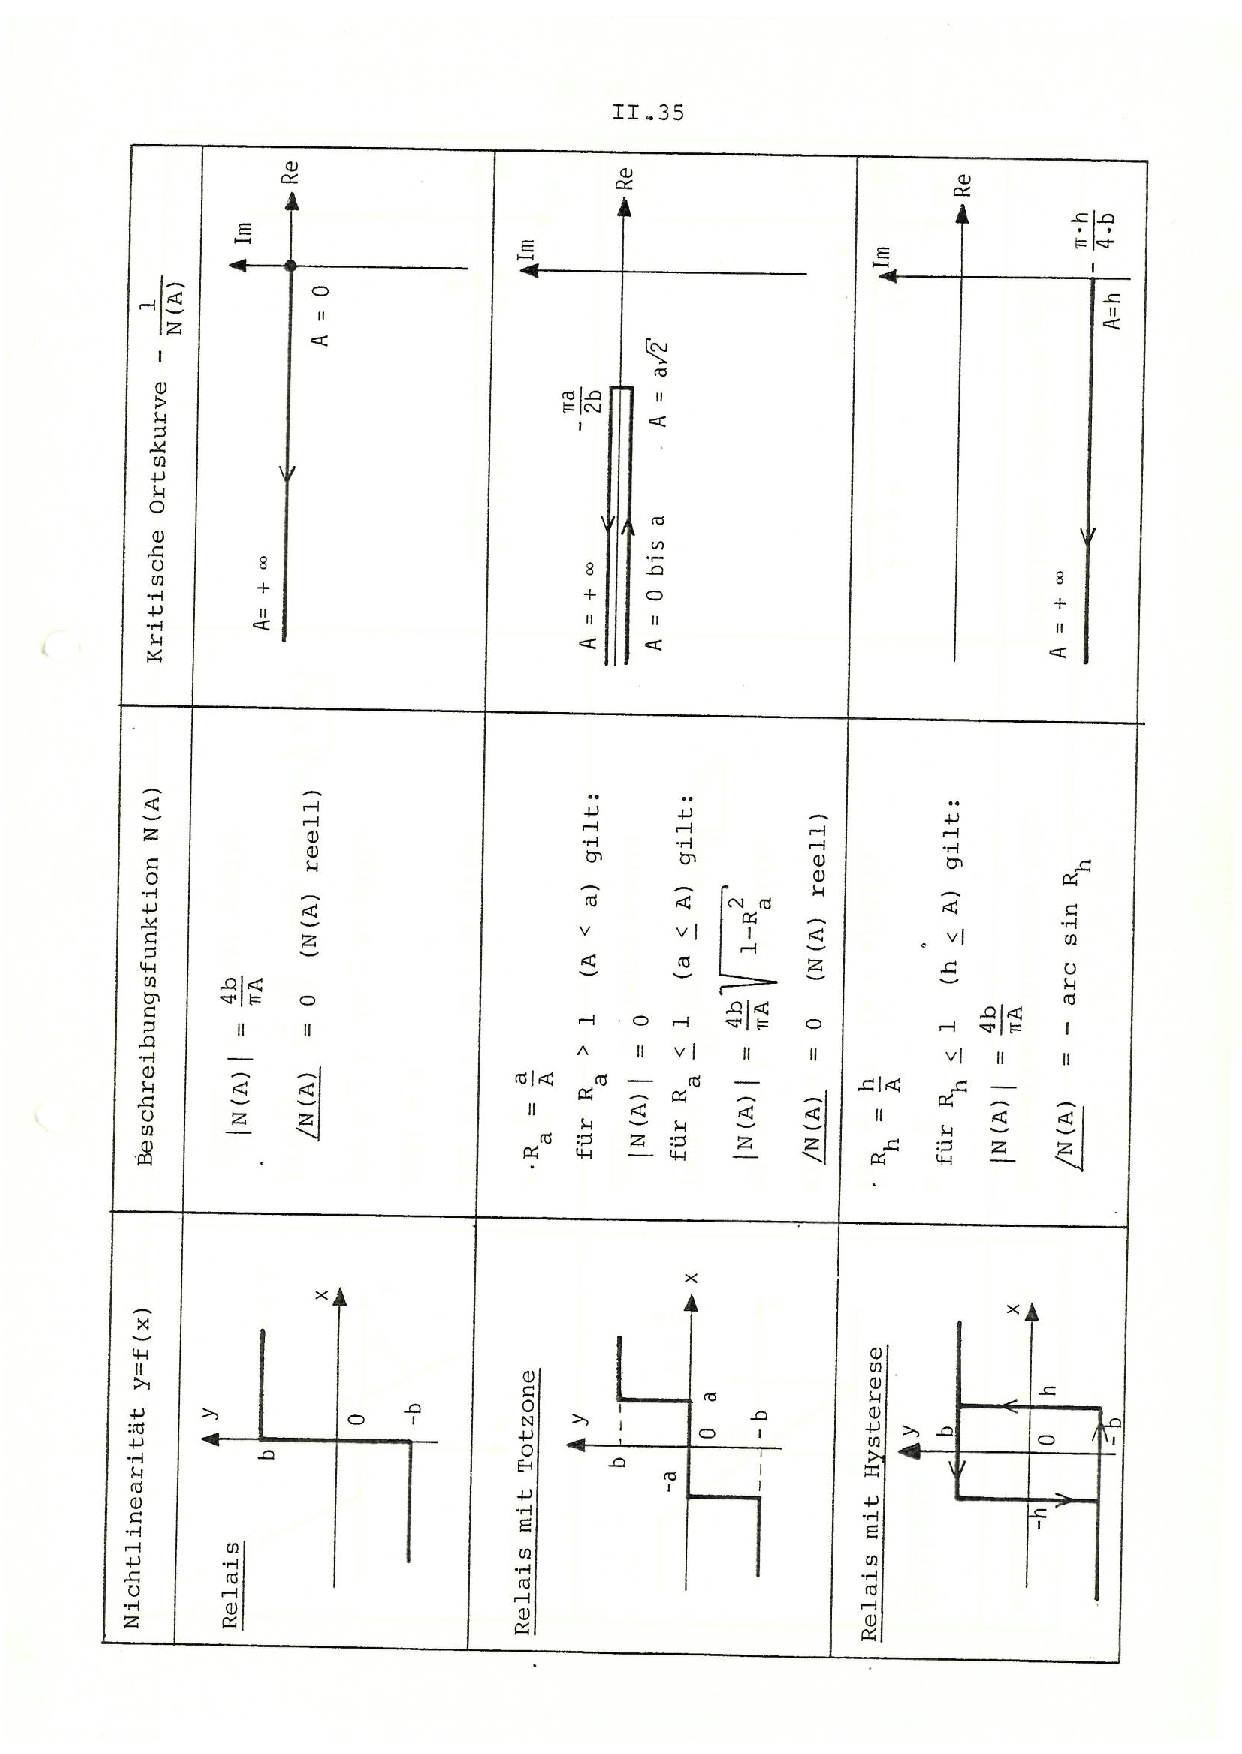
\includepdf[angle=1.23,pages=1,scale=0.95]{./Anhang/describingFunctions}
\end{minipage}
\newpage
\begin{minipage}{\linewidth}
	\includepdf[angle=0.285,pages=2,scale=0.95]{./Anhang/describingFunctions}
\end{minipage}
\newpage
\begin{minipage}{\linewidth}
	\includepdf[angle=1.85,pages=3,scale=0.95]{./Anhang/describingFunctions}
\end{minipage}
\newpage
\begin{minipage}{\linewidth}
	\includepdf[angle=0.815,pages=4,scale=0.95]{./Anhang/describingFunctions}
\end{minipage}

\end{document}
